\chapter{与 AI 一起推演构图和草图}
\usetikzlibrary{decorations.pathreplacing}

分子生物学博士生林悦正在准备学位论文开题报告，同时为一篇基因组编辑综述撰写引言。她需要制作全篇的第一张总览图（Figure 1），向跨细分方向的生命科学同行与评审交代化脓链球菌 Cas9（SpCas9）如何在单链引导 RNA（sgRNA）引导下识别原间隔序列邻近基序（PAM）并切开双链 DNA，以及非同源末端连接（NHEJ）与同源定向修复（HDR）两条主要修复途径如何决定不同的编辑结局。

她打开图像生成工具，输入了一句看似省事的指令：“画一张专业、有视觉冲击力的 CRISPR–Cas9 基因编辑机制总览图，适合顶刊发表。”几十秒后，工具生成了一张色彩饱满的横版插图：深蓝色的立体细胞核背景中央悬着一把发着青光的剪刀，正在剪断一条扭曲的三维双螺旋 DNA；画面的四个角落散落着一段飘带状的 RNA、一枚标着“PAM”的发光徽章，以及两段分别带有裂痕和彩色补丁的短双链。

林悦觉得画面的光影质感远超自己用基础绘图软件拼出的线框，便直接放进了开题幻灯片。没想到导师看了一眼屏幕，只用了五秒钟就问出一句话：“这张图应该从哪里开始看？”

林悦一时语塞。导师接着指着屏幕追问：读者的第一眼会被正中央最大的发光剪刀吸引过去，可切割双链明明是第三步；看完剪刀之后，视线该往左上角找 RNA，还是往右下角看修复结果？左下角和右下角的两段 DNA 之间既没有连线也没有基线对齐，读者怎么知道它们是由同一个断裂分出来的两条并列修复途径，而不是一前一后的两个步骤？

这张初稿的问题不在画功，而在于作者点击“生成”按钮之前，没有替读者决定视线的落脚点与行进路线。只要输入中缺少明确的构图骨架，模型就会按照装饰画的对称习惯把元素随机摊在画布上，让读者的视线在四个角落之间来回乱撞。本章把构图推演与草图设计提前到精细渲染之前，依次解决五个问题：如何用“入口—路径—终点”控制阅读顺序，如何判断哪些内容应该放进同一个面板，如何针对同一份任务书画出三种结构不同的草图骨架，如何在 \scidraw{} 中由草图生成候选图并按写明的标准做出选择，以及如何用“每次只改一个可核对目标”的纪律完成定稿。

\section{读者的视线先于画面}

审稿人或读者翻开论文看到一张总览图时，并不是像读正文那样逐字扫描，而是在最初几秒钟内先靠视觉本能寻找落脚点，再顺着画面提供的几何线索往下走（Wong，2011c；Rougier 等，2014）。如果一张图不能在前五秒内让读者看懂“从哪开始、往哪走、最后停在哪”，里面的分子局部画得再精致，也会在读图时制造理解阻力。

在动笔或输入提示词之前，作者应当先用三个问题替读者规划好视线轨迹：

\begin{itemize}
\item \textbf{第一，入口在哪里？} 读者的第一眼必然落在画面中视觉权重最大的地方——通常是面积最大、明度或色彩对比最高、造型最孤立，或者位于日常阅读习惯起点（横排出版物为左上角或左端）的元素。如果一张图没有安排明确的入口，或者同时摆放了三四个尺寸相当、对比度都很强烈的团块，读者在进入画面的瞬间就会陷入犹豫。
\item \textbf{第二，路径怎么走？} 进入画面之后，视线需要明确的几何向导。最直接的向导是单向箭头和步骤编号（1、2、3……）；更底层也更稳定的向导则是元素的水平与垂直对齐基线、连续留白形成的通道，以及顺应阅读习惯的推进方向（从左到右、从上到下）。
\item \textbf{第三，终点停在哪里？} 视线走完路径停驻的位置，应当恰好承载这张图最核心的科学结论。在包含因果或时间链条的总览图中，如果把上游的常见背景组件画得硕大无比，而把真正需要读者比对的实验结局或修复结果挤在角落里，就会造成头重脚轻，让主要信息沦为视觉附庸。
\end{itemize}

\begin{figure}[htbp]\centering
\resizebox{\linewidth}{!}{% FIG ch03-01 reading order (Chinese)
\begin{tikzpicture}[
  x=1mm, y=1mm,
  font=\sffamily\footnotesize,
  panel/.style={draw=BookInk!40, line width=0.3pt, rounded corners=1pt},
  block/.style={
    rounded corners=2pt, draw=black!60, fill=black!5,
    minimum size=7mm, inner sep=0pt, font=\sffamily\footnotesize,
  },
  eye/.style={line width=4pt, draw=blue!50, opacity=0.35, rounded corners=2pt},
  paneltitle/.style={font=\sffamily\scriptsize, text=BookInk, align=center},
]
  \def\pw{50}\def\ph{35}
  \begin{scope}[shift={(0,42)}]
    \draw[panel] (0,0) rectangle (\pw,\ph);
    \node[paneltitle, anchor=north] at (0.5*\pw,\ph+2.5) {(a) 线性};
  \end{scope}
  \begin{scope}[shift={(54,42)}]
    \draw[panel] (0,0) rectangle (\pw,\ph);
    \node[paneltitle, anchor=north] at (0.5*\pw,\ph+2.5) {(b) 中心辐射};
  \end{scope}
  \begin{scope}[shift={(108,42)}]
    \draw[panel] (0,0) rectangle (\pw,\ph);
    \node[paneltitle, anchor=north] at (0.5*\pw,\ph+2.5) {(c) 两分支};
  \end{scope}
  % (a) linear 1-5
  \begin{scope}[shift={(0,42)}]
    \foreach \i/\x in {1/8,2/18,3/28,4/38,5/42} {
      \node[block] at (\x,17.5) {\i};
    }
    \draw[eye] (6,22) .. controls (15,26) and (35,26) .. (44,22);
    \foreach \i/\xa/\xb in {1/11/15,2/21/25,3/31/35,4/41/45} {
      \draw[-{Stealth[length=1.2mm]}, draw=BookInk!35, thin] (\xa,17.5) -- (\xb,17.5);
    }
  \end{scope}
  % (b) hub
  \begin{scope}[shift={(54,42)}]
    \node[block] at (25,17.5) {3};
    \node[block, minimum size=5.5mm] at (8,28) {1};
    \node[block, minimum size=5.5mm] at (42,28) {2};
    \node[block, minimum size=5.5mm] at (8,7) {4};
    \node[block, minimum size=5.5mm] at (42,7) {5};
    \draw[eye, blue!50] (25,20) .. controls (32,26) .. (42,28);
    \draw[eye, orange!70!black, opacity=0.35] (25,20) .. controls (18,26) .. (8,28);
    \draw[eye, blue!50] (25,15) .. controls (32,8) .. (42,7);
    \node[font=\Large, text=BookInk!60] at (32,17) {?};
  \end{scope}
  % (c) two-branch
  \begin{scope}[shift={(108,42)}]
    \foreach \i/\x in {1/10,2/25,3/40} {
      \node[block, minimum size=6mm] at (\x,28) {\i};
    }
    \node[block, minimum size=6mm] at (25,12) {4};
    \node[block, minimum size=6mm] at (25,5) {5};
    \draw[-{Stealth[length=1mm]}, draw=BookInk!35, thin] (13,28) -- (22,28);
    \draw[-{Stealth[length=1mm]}, draw=BookInk!35, thin] (28,28) -- (37,28);
    \draw[-{Stealth[length=1mm]}, draw=BookInk!35, thin] (40,26) -- (40,20) -- (25,20) -- (25,15);
    \draw[-{Stealth[length=1mm]}, draw=BookInk!35, thin] (25,20) -- (25,8);
    \draw[eye] (8,30) .. controls (18,32) .. (38,30) .. controls (42,22) .. (25,14);
    \draw[eye] (25,14) -- (25,6);
  \end{scope}
  % bottom row: proximity, alignment, enclosure, hierarchy
  \def\bw{38}\def\bh{22}
  \foreach \i/\x/\title in {
    1/0/接近, 2/42/对齐, 3/84/围合, 4/126/主次} {
    \begin{scope}[shift={(\x,0)}]
      \draw[panel] (0,0) rectangle (\bw,\bh);
      \node[paneltitle, anchor=north] at (0.5*\bw,-2.5) {\title};
    \end{scope}
  }
  \begin{scope}[shift={(0,0)}]
    \foreach \x in {6,10,14} {\fill[BookInk] (\x,14) circle (0.9mm);}
    \foreach \x in {26,30,34} {\fill[BookInk] (\x,14) circle (0.9mm);}
  \end{scope}
  \begin{scope}[shift={(42,0)}]
    \draw[fill=BookInk!15, draw=BookInk!50] (4,6) rectangle (16,18);
    \draw[fill=BookInk!15, draw=BookInk!50] (4,6) rectangle (14,18);
    \node[font=\scriptsize, anchor=west] at (18,12) {对齐};
    \node[font=\scriptsize, anchor=west, text=BookInk!55] at (18,7) {不对齐};
  \end{scope}
  \begin{scope}[shift={(84,0)}]
    \draw[fill=BookRule!40, rounded corners=2pt] (3,5) rectangle (35,19);
    \foreach \x in {10,19,28} {
      \draw[fill=BookPale, draw=BookInk!40, rounded corners=1pt] (\x-3,9) rectangle (\x+3,15);
    }
  \end{scope}
  \begin{scope}[shift={(126,0)}]
    \draw[fill=BookInk!25, draw=BookInk!60, rounded corners=2pt] (14,6) rectangle (26,18);
    \foreach \x/\y in {6/16,6/10,32/16,32/10} {
      \draw[fill=BookInk!8, draw=BookInk!45, rounded corners=1pt] (\x-2.5,\y-2) rectangle (\x+2.5,\y+2);
    }
  \end{scope}
\end{tikzpicture}
}
\caption{阅读顺序由布局决定。上：同样五个元素按三种结构排列，半透明曲线表示读者最可能的视线路径；中心辐射式没有唯一入口，读者可能沿不同路径阅读。下：控制主次与分组的四种基本手段。}\label{fig:ch03-01}
\end{figure}

图~\ref{fig:ch03-01} 上排展示了同样五个事件节点（编号 1 至 5）在三种不同布局结构下的视线走向。在图~\ref{fig:ch03-01}a 的\textbf{线性布局}中，五个圆角方块从左到右排成一行，由灰色细箭头相连；半透明蓝色粗曲线标出了毫无歧义的视线路径——从左端节点 1 进入，顺着箭头一路向右，在右端节点 5 结束。这种结构天然契合单一时间序列或单向实验流程。

再看图~\ref{fig:ch03-01}b 的\textbf{中心辐射布局}。节点 3 被放在画布正中央且尺寸较大，节点 1、2、4、5 分散在四个角落。这种排法在头脑风暴或概念关联图中很常见，但一旦用于表达有先后顺序的科学过程，就会立刻制造阅读障碍：图中叠加的蓝色与橙色两条半透明曲线表明，不同读者会走出截然不同的路径——有人先被正中央的节点 3 吸引，随后随机跳向右上角的 2 或右下角的 5；有人习惯性地先看左上角的 1，经过中央的 3 之后却不知道下一步该去右上角还是左下角。中央旁边的问号标出了这种决策困惑：当画面缺乏唯一入口且四周节点地位均等时，读者只能靠猜来拼凑事件顺序。

图~\ref{fig:ch03-01}c 则展示了适合表达“共同上游、两种结局”的\textbf{两分支布局}。节点 1、2、3 在上排从左到右紧凑排列，交代共同前提步骤；从节点 3 向下引出分叉箭头，接入下方上下并列的节点 4 与节点 5。读者的视线先沿上排完成水平扫描，随后顺着分叉箭头向下进入并列对比区，既不会弄混上游与下游的先后次序，又能直观看出 4 和 5 是由同一个节点 3 分化出来的两条平行支路。

看清了骨架对路径的控制作用，下一步是掌握调控画面内部秩序的四项基本视觉手段（图~\ref{fig:ch03-01} 下排）。前三项直接源自格式塔（Gestalt）视觉感知原则（Wong，2010a，2010b），第四项则是构建视觉层级的核心法则（Wong，2011d）：

\begin{enumerate}
\item \textbf{接近（Proximity）：} 空间距离相近的元素会被大脑自动归为同一组。如图~\ref{fig:ch03-01} 下排左一所示，六个完全相同的圆点不需要任何边框，仅靠“组内间距小、组间间距大”就自然分成了左右两群。在科研图中，成片的留白（负空间）绝不是浪费版面，而是分隔不同实验阶段或不同分子复合物的隐形隔板（Wong，2011b）。当生成模型把所有分子均匀铺满整张画布时，正是因为丧失了“接近与留白”的间距对比，读者才会觉得画面乱成一团。
\item \textbf{对齐（Alignment）：} 共享同一水平基线或垂直左边界的元素，会被读者视为处于同一结构层级或具备直接可比性（图~\ref{fig:ch03-01} 下排左二）。在对比两种修复结果或两组处理前后状态时，把两条 DNA 双链的左右端点严格对齐，读者一眼就能锁定中间发生改变的片段；反之，如果两条链一长一短、一左一右错开摆放，读者就会分心去猜这种错位是否代表序列发生了截短或位移。
\item \textbf{围合（Enclosure）：} 用浅色底框或细线矩形把若干元素框在同一个边界内，是力度最强的分组方式（图~\ref{fig:ch03-01} 下排左三）。当一条修复通路内部同时包含断裂底物、外源供体模板与修复后产物时，用一个简洁的矩形通道框把它们围合起来，就能明确宣告这些元素同属一个修复方案，防止悬浮的供体模板被误认为属于隔壁通道。
\item \textbf{主次（Hierarchy）：} 一张图只能有一个视觉最重的中心（图~\ref{fig:ch03-01} 下排右一）。许多作者习惯用“加更多鲜艳颜色”来强调重点，结果每个对象都涂得五彩斑斓，反而互相抵消。分配视觉权重的稳妥做法是组合运用\textbf{尺寸、明度对比和空间位置}：把最重要的结论对比区画得最大、留白最舒展，用高对比度色彩只标出关键变化位点（如几碱基的切口或写入片段），而将未改变的背景骨架压低为柔和的中性灰色。
\end{enumerate}

把上述四项手段合起来，可以浓缩成一条构图铁律：\textbf{分组即声明——凡是在画面上靠在一起、对齐在一处、框在同一框内或涂成同一种颜色的对象，读者都会默认它们在科学逻辑上彼此相关。} 同样，版面的推进方向也是声明：横排论文图应让因果或时间链条顺着“从左到右”或“从上到下”的自然阅读方向展开；遇到分支选择时，必须把两条支路画成几何对称或上下并列的等权通道，切忌把其中一条画成主干直行、另一条画成旁支折返，否则读者会把并列选项误读为主次或先后关系。

在把构图交给精修之前，可以用三个简单动作做一次快速自测：第一是\textbf{五秒测试}，把草图或初稿给一位没看过任务书的同事看五秒钟后收起，请对方说出第一眼看到什么、这张图主要在比较什么；第二是\textbf{手指描路径}，请同事用手指在图上从第一眼看到的位置描到最后看的位置，凡是手指停顿、画圈或往回折返的地方，就是构图线索断裂之处；第三是\textbf{缩略图与灰度检查}，把图片缩放到目标印刷宽度（如通栏 174 mm）的 50\% 并转为灰度，检查是否仍然只有一个清晰的视觉重心，以及不同步骤之间的留白通道是否贯通。

\section{什么值得放在同一面板}

确立了阅读顺序原则后，接下来要解决“画多少”的问题。科研总览图最容易犯的第二个通病是贪多求全：作者生怕审稿人觉得背景交代不完整，试图在同一个面板里从质粒或核糖核蛋白（RNP）递送跨过细胞膜画起，穿过核孔进入细胞核，画出整条染色体和核小体解旋，再画 Cas9 蛋白的写实三维晶体结构、HNH 与 RuvC 两个催化结构域的氨基酸位点，接着往下塞进 Ku70/80、DNA-PKcs、连接酶 IV 等一整串修复因子，顺手还要在角落里补上脱靶效应、微同源介导末端连接（MMEJ）乃至碱基编辑。结果一张 174 mm 宽的图被塞进三四十个尺度悬殊的对象，既看不清宏观路径，也核对不了微观几何。

决定哪些内容应该放进同一个面板，判据只有一条：\textbf{一个面板只回答一个核心问题；只有读者必须同时看到、放在一起比对才能理解因果链条或结局差异的内容，才应该放进同一个面板。}

回到本章林悦的 CRISPR–Cas9 基因组编辑总览图案例。按照第一章确立的“一句话目标模板”，她首先把这张 Figure 1 要回答的问题写成一句可核查的任务陈述：

\begin{BookNote}
看完这张图，读者应该能够理解\textbf{单链引导 RNA（sgRNA）引导 Cas9 识别紧邻 PAM 的靶序列并在该处产生双链断裂，随后非同源末端连接（NHEJ）与同源定向修复（HDR）两种修复途径分别产生不精确的小片段插入/缺失或按供体模板的精确编辑}，并能从图中找到\textbf{事件的先后顺序、PAM 与切点的相对位置，以及两种结果在 DNA 序列层面的差别}。
\end{BookNote}

这张总览图不报告作者本人的实验测量数据，也不包含尚未证实的新假说，其全部内容均建立在基因组编辑领域已确立的教科书与经典研究共识之上：Jinek 等（2012）证实化脓链球菌 Cas9 是由双 RNA（或人工融合的 sgRNA）引导的 DNA 内切酶，依赖非靶链上的 PAM 识别靶位点，并通过 HNH 与 RuvC 样两个核酸酶结构域分别切割互补靶链与非靶链；Ran 等（2013）明确了 SpCas9 识别 $5'$-NGG-$3'$ PAM 并在其上游约 3 个碱基对（bp）处产生双链断裂的实验设计准则；Doudna 与 Charpentier（2014）以及 Hsu 等（2014）系统总结了双链断裂后细胞通过 NHEJ 或 HDR 进行修复的总体框架及两类编辑结局；Chang 等（2017）则对 NHEJ 及替代末端连接途径的分子机制与连接保真度做了严谨界定。

动笔绘制任何草图之前，作者先把上述文献共识整理成九条可逐项核验的关系表（表~\ref{tab:ch03-01-rel}，编号 C1 至 C9）。

\begin{table}[htbp]\centering\footnotesize
\setlength{\tabcolsep}{3pt}
\renewcommand{\arraystretch}{1.15}
\caption{CRISPR–Cas9 基因组编辑总览图的关系表（C1–C9）。所有关系均为教科书与综述层面的确立共识；简化之处须在图注中声明。}\label{tab:ch03-01-rel}
\begin{tabularx}{\linewidth}{@{}l>{\raggedright\arraybackslash}p{25mm}>{\raggedright\arraybackslash}p{25mm}>{\raggedright\arraybackslash}p{18mm}Y@{}}
\toprule
\textbf{\#} & \textbf{起点} & \textbf{终点 / 结果} & \textbf{关系与状态} & \textbf{本图简化说明} \\
\midrule
C1 & sgRNA（crRNA:tracrRNA 融合链） & Cas9 蛋白 & 结合形成复合物（确立） & 不画 sgRNA 二级结构细节，简化为带间隔段与发夹支架的 RNA 链 \\
C2 & Cas9–sgRNA 复合物 & 基因组 DNA 上的 PAM（SpCas9 为 $5'$-NGG-$3'$） & 识别 PAM（确立） & 不画 Cas9 沿 DNA 搜索的中间过程 \\
C3 & sgRNA 间隔序列（约 20 nt） & 靶链（与间隔序列互补的 DNA 链） & 碱基配对形成 R 环，非靶链被置换（确立） & 不画 R 环分步形成的动力学过程 \\
C4 & PAM 的空间位置 & 非靶链上、紧邻原间隔序列 $3'$ 端 & 链极性与空间邻接（确立） & 主面板只画黄色高亮小段；精确链方向与极性放入插图 \\
C5 & Cas9（HNH 与 RuvC 样结构域） & 两条链在 PAM 上游约 3 bp 处被切开 & 产生双链断裂，多为平末端（确立） & 主面板不区分两个结构域；插图中明确区分 HNH 与 RuvC \\
C6 & 双链断裂 & NHEJ（非同源末端连接） & 修复途径之一，不需要模板（确立） & 不画 Ku70/80、DNA-PKcs、连接酶 IV 等因子；不画 MMEJ 等替代途径 \\
C7 & NHEJ 修复过程 & 断裂处可能出现小片段插入或缺失（indel） & 结果；位于编码区时可致移码失活（确立） & 用“可能”表述；NHEJ 也可准确连接并被再次切割，图中省略该循环 \\
C8 & 双链断裂 + 外源供体模板（带同源臂） & HDR（同源定向修复） & 修复途径之一，需要模板（确立） & 不画末端切除、链入侵等中间步骤 \\
C9 & HDR 修复过程 & 按供体模板写入的精确改变（插入或替换） & 结果；在多数细胞中频率低于 NHEJ（确立） & 不给任何效率数值；“频率较低、主要发生在 S/G2 期”只在图注中写 \\
\bottomrule
\end{tabularx}
\end{table}

审视表~\ref{tab:ch03-01-rel}，有两处科学表述细节需要特别注意。第一，在 C7 中，我们把 NHEJ 的结局写为“断裂处\textbf{可能}出现小片段插入或缺失”，而不把 NHEJ 简单贴上“必然出错”的标签。正如 Chang 等（2017）所指出的，经典 NHEJ 本身具有较高的连接保真度；在基因编辑实验中之所以常观察到 indel，是因为准确重连后的原序列仍保有完整的靶位点与 PAM，会被持续存在的 Cas9–sgRNA 再次切割，直到末端产生 indel 破坏识别位点为止。总览图虽为简洁省略了“准确重连—再次切割”的循环，但文字表述必须保留“可能”。第二，在 C9 中，HDR 的效率取决于细胞类型、细胞周期（主要在 S/G2 期）与供体设计，总览图中绝不给出任何脱离实验条件的百分比数字。

对照目标句与表~\ref{tab:ch03-01-rel}，我们可以对全部素材做一次清晰的“三路分流”：

\begin{itemize}
\item \textbf{第一路：保留在总览主面板。} 主面板只负责交代“谁参与、在哪里、先后顺序如何、产生哪两种结果”，仅保留八类核心对象：Cas9 双叶轮廓、橙色 sgRNA、梯状双链 DNA、黄色 PAM 小段、双链断裂缺口、带同源臂与青绿中段的短双链供体模板，以及 NHEJ（带红紫 indel 标记）和 HDR（带青绿写入段）两条结果 DNA。
\item \textbf{第二路：拆入细节插图（Inset）。} 目标句要求读者找到“PAM 与切点的相对位置”。这一信息涉及分子尺度的精确几何关系：靶链与非靶链的 $5'\rightarrow 3'$ 反向平行极性、PAM（$5'$-NGG-$3'$）位于非靶链紧邻原间隔序列 $3'$ 侧、sgRNA 约 20 nt 间隔序列与靶链配对、切点位于 PAM 上游约 3 bp 处，以及 HNH 切割靶链、RuvC 样结构域切割非靶链的分工。把这些微观几何拆成独立插图，既免去了主面板的拥挤，又能把碱基位置交代得一清二楚。
\item \textbf{第三路：坚决删去，在图注中声明省略。} 细胞与细胞核轮廓、染色体、递送方式（质粒、RNP、病毒）、Cas9 的写实三维结构、NHEJ 与 HDR 的分子因子、替代末端连接途径、脱靶切割、碱基编辑与先导编辑等其他系统，以及任何效率数值，统统不画，并在图注末尾集中声明省略。
\end{itemize}

\begin{figure}[htbp]\centering
% FIG ch03-07 PAM inset (Chinese)
\begin{tikzpicture}[
  x=1mm, y=1mm,
  font=\sffamily\scriptsize,
  text=BookInk,
]
  \node[anchor=east] at (-2, 21.2) {非靶链};
  \node[anchor=east] at (-2, 7.2) {靶链};
  \node at (6, 23.6) {5$'$};
  \node at (54.5, 23.6) {3$'$};
  \node at (55.5, 4.4) {5$'$};
  \node at (6, 4.4) {3$'$};

  \foreach \i in {0,...,19} {
    \pgfmathsetmacro{\x}{6+\i*2.4}
    \draw[draw=BookInk!50, fill=white] (\x,20) rectangle (\x+2.4,22.4);
  }
  \foreach \i in {0,1,2} {
    \pgfmathsetmacro{\x}{6+(17+\i)*2.4}
    \draw[draw=BookInk!50, fill=yellow!70] (\x,20) rectangle (\x+2.4,22.4);
  }
  \node[anchor=west, text=BookInk!80] at (6+17*2.4, 28.2) {PAM（NGG）};

  \foreach \i in {0,...,19} {
    \pgfmathsetmacro{\x}{6+\i*2.4}
    \draw[draw=BookInk!50, fill=white] (\x,6) rectangle (\x+2.4,8.4);
  }
  \foreach \i in {0,...,19} {
    \pgfmathsetmacro{\x}{6+\i*2.4}
    \draw[BookInk!35, thin] (\x+1.2,8.4) -- (\x+1.2,11.6);
    \draw[draw=orange!80!black, fill=orange!25, line width=1pt]
      (\x,4) rectangle (\x+2.4,6.4);
  }
  \draw[orange!80!black, line width=0.8pt]
    (6+19*2.4+2.4, 5) .. controls (6+21*2.4, 8) .. (6+21*2.4, 12)
    .. controls (6+21*2.4, 14) .. (6+19*2.4, 14);

  \node[anchor=west] at (6, 0.5) {sgRNA 间隔序列};
  \pgfmathsetmacro{\cx}{6+16.5*2.4+1.2}
  \fill[black] (\cx,20) -- (\cx-0.8,21.2) -- (\cx+0.8,21.2) -- cycle;
  \fill[black] (\cx,6) -- (\cx-0.8,4.8) -- (\cx+0.8,4.8) -- cycle;
  \node[anchor=west] at (6+17.5*2.4, 13) {切点};
  \node[anchor=west, font=\scriptsize] at (6+16*2.4, 17) {RuvC};
  \node[anchor=west, font=\scriptsize] at (6+16*2.4, 3) {HNH};

  \draw[decorate, decoration={brace, amplitude=3pt}] (6, 15.5) -- (6+20*2.4, 15.5)
    node[midway, above=4pt] {约 20 nt};
  \draw[decorate, decoration={brace, amplitude=2pt, mirror}] (6+16*2.4, 22.5) -- (6+17*2.4, 22.5)
    node[midway, below=2pt] {3 bp};
\end{tikzpicture}

\caption{PAM 与切点的相对位置（SpCas9）。sgRNA 间隔序列与靶链配对；PAM（$5'$-NGG-$3'$）位于非靶链上原间隔序列的 $3'$ 侧；两条链在 PAM 上游约 3 bp 处被切开，HNH 结构域切割靶链，RuvC 样结构域切割非靶链。示意图，序列长度未按比例。}\label{fig:ch03-07}
\end{figure}

把微观细节拆成插图还有一个直接关乎工具选择的理由：\textbf{精确几何关系（链方向、PAM 所在链、切点距离）不适合交给图像生成模型，而必须用确定性绘图工具制作。} 图像模型并不理解双链反向平行规则，常把 $5'$ 和 $3'$ 标在同一端、把 PAM 画错链，或在距离 PAM 任意远的地方随机断开。

图~\ref{fig:ch03-07} 展示了用确定性代码（TikZ）绘制的 PAM 与切点插图：上链为非靶链（左 $5'$、右 $3'$），下链为靶链（左 $3'$、右 $5'$）；下方橙色 sgRNA 间隔段通过短竖线与下链靶链的 20 个方格逐格配对，并在 $3'$ 端接简化发夹支架；上链非靶链紧邻配对区 $3'$ 侧的三个方格涂为黄色并标注“PAM（NGG）”；切点用两个黑色实心小三角精确放在 PAM 左侧第 3 与第 4 格之间（即上游 3 bp 处），上链标 RuvC、下链标 HNH（依据 Jinek 等，2012）。这幅确定性插图将在第 6 节直接嵌入总览图终稿的右上角空白区。

\section{从文字到草图：先画三种骨架}

完成取舍与关系表后，先把以下任务书保存在自己的文档里（三张候选图共用这份任务书，只换草图）；再在 \scidraw{} 科研绘图向导（\sdtool{figure-workflow}）选“机制图 / 流程图”，按路线进入第 1 步的机制图生成（\sdtool{mechanism-figure-generator}），把任务书粘贴进去：

\begin{Prompt}
【用途与读者】开题报告与综述引言的 Figure 1 总览示意图，双栏通栏宽 174 mm、高约 110 mm；读者为了解分子生物学基础、但未必做过基因编辑的同行与评审。
【目标】让读者按顺序看清：sgRNA 与 Cas9 结合 → 复合物识别 DNA 上的 PAM、间隔序列与靶链配对 → 在 PAM 上游切开两条链形成双链断裂 → 两种修复途径（NHEJ：不需模板，可能留下小片段插入/缺失；HDR：需供体模板，得到精确编辑）。主要信息是“同一个断裂，两种修复，两种结果”。
【材料】教科书与综述层面的已确立关系（Jinek 2012；Doudna & Charpentier 2014；Hsu, Lander & Zhang 2014；Ran 等 2013）。不含作者数据。
【对象】Cas9（一个圆润的双叶蛋白轮廓）；sgRNA（一条 RNA 链，含间隔段与发夹支架）；基因组 DNA（双链，用两条平行线及横档表示）；PAM（DNA 上一小段高亮）；双链断裂（DNA 上的缺口）；供体模板（一段短双链 DNA，两端为同源臂，中间为待写入的片段）；修复后的 DNA 两条（NHEJ 结果、HDR 结果）。每个对象只出现一次，DNA 在每个步骤中各出现一段。
【关系】按关系表 C1–C9。步骤之间用同一种实线箭头；断裂处分叉为两条并列箭头，分别通往 NHEJ 与 HDR；供体模板只出现在 HDR 通道中，并与断裂位置对齐。
【布局】按所附草图的结构；三种候选图分别对应草图 A（线性）、B（中心辐射）、C（两分支）。底部 10% 留空。
【视觉】白底、扁平二维、细深灰描边，无渐变、阴影、3D。颜色角色：Cas9 蓝灰；sgRNA 橙；DNA 深灰；PAM 黄；供体模板与 HDR 写入片段青绿；NHEJ 的 indel 位置用小红紫标记。全图不超过 4 个色相加灰色。对象之间留出标签空间。
【限制】底图中不出现任何文字、字母、数字或符号；不画细胞、细胞核、染色体、病毒、剪刀、闪电、发光效果；不画 Cas9 的写实三维结构；不画数据或图表。
【图例】在 LaTeX 中制作：实线箭头=步骤；分叉箭头=两种可选修复途径；黄色=PAM；红紫标记=indel；青绿=供体模板来源的序列。
【验收】C1–C9 逐条可找到；PAM 在断裂的同一侧且紧邻；供体模板只在 HDR 通道；两条结果通道的 DNA 长度、位置一致以便对照；阅读顺序可用 1–5 编号无歧义标出；底图无文字；174 mm 宽下叠加 7 pt 标签后可读。
\end{Prompt}

为什么不能只凭文字提示词让工具一次生成四张图来挑选？因为\textbf{同一提示词批量生成的候选共享同一文本先验，变化主要停留在局部造型、笔触和配色深浅上，而不会替你主动规划截然不同的版面结构}。作者可以先请对话式 AI 根据任务书用文字建议几种布局骨架及各自的阅读顺序，但文字建议只是概念；要把空间分区、相对大小和流向真正固定下来，必须由作者画出至少三种结构不同的\textbf{骨架草图}：

\begin{itemize}
\item \textbf{骨架 A（线性左 $\rightarrow$ 右）：} 把全部步骤沿水平方向排成单行，最右端分出上下两个小箭头指向两条短结果双链。
\item \textbf{骨架 B（中心辐射）：} 把结合在 DNA 上的 Cas9–sgRNA 复合物放在正中央，将 sgRNA、PAM 细节、NHEJ 结果与 HDR 结果分散放在四角，用两进两出的单头箭头连接。
\item \textbf{骨架 C（两分支结果）：} 上三分之一紧凑排列“结合 $\rightarrow$ 识别配对 $\rightarrow$ 双链断裂”三步；从第三步向下引出分叉箭头，进入下方上下堆叠的两条宽水平通道（上通道为 NHEJ，下通道为带短供体的 HDR），两条长 DNA 左右端点严格对齐。
\end{itemize}

草图要画什么、不画什么？原则很清楚：\textbf{只画分区边界、相对大小、箭头方向与底部约 10\% 的留白；不画分子细节，更不写任何文字、字母或数字。} 一旦在草图上写了手写字，图像模型很容易把笔迹当成图案原位重绘成乱码（若需标阅读顺序编号，可在后期用排版层叠加）。日常作图中鼓励读者直接用铅笔在纸上手绘拍照；本书用图像模型模拟了这三张铅笔草图（图~\ref{fig:ch03-02}），共用如下开头提示词：

\begin{Prompt}
A rough pencil planning sketch on slightly off-white sketchbook paper, photographed flat from directly above, evenly lit, no hands, no pencil, no other objects. Landscape 16:9. Single graphite pencil, loose confident lines, a few construction lines and faint erasure marks. Simple shapes only: rounded blobs, pairs of parallel lines with short rungs (double-stranded DNA), a wavy line (RNA), arrows. Strictly no writing of any kind: no letters, no words, no numbers, no labels, no title, no annotations. Pencil gray only, no color. Bottom tenth of the page left blank.
\end{Prompt}

随后分别拼接三种骨架的布局描述段：

\begin{Prompt}
[A - Linear] Layout: one horizontal row of four steps from left to right, connected by short arrows. Step 1 at far left: a rounded two-lobed blob with a short wavy line tucked inside it. Step 2: a horizontal ladder-like double line with the same blob sitting on it; a small shaded rectangle on the upper line at the right edge of the blob. Step 3: the double line with a clear gap cut through both lines, the small shaded rectangle right next to the gap. Step 4 at far right, squeezed: the arrow splits into two small arrows, one going up-right and one going down-right, each ending at a short double line; the lower one has a small separate short double line floating above it.
\end{Prompt}

\begin{Prompt}
[B - Hub] Layout: radial. In the exact center, a large rounded two-lobed blob sitting on a short ladder-like double line. Around it, at the four corners of the page, four smaller shapes: top-left a short wavy line, top-right a small shaded rectangle on a short double line, bottom-left a short double line with a tiny zigzag mark, bottom-right a short double line with a short thick inserted segment and a separate short double line above it. Arrows connect the center to each corner: two arrows point inward, two point outward. No clear starting point.
\end{Prompt}

\begin{Prompt}
[C - Two-branch] Layout: two tiers. Upper third of the page: a compact row of three small steps from left to right connected by arrows (a two-lobed blob with a wavy line inside; the blob sitting on a ladder-like double line with a small shaded rectangle; the double line with a gap through both lines, the shaded rectangle right next to the gap). From the third step, one arrow goes down and splits into two arrows. Lower part of the page: two wide horizontal lanes of equal height, stacked one above the other, each framed by a light pencil rectangle. Upper lane: a long double line with a tiny zigzag mark at the middle. Lower lane: a short separate double line floating above the middle of a long double line, and the long double line has a short thick inserted segment at the middle. The long double lines in both lanes start and end at the same x positions.
\end{Prompt}

\begin{figure}[htbp]\centering
\begin{minipage}[t]{0.32\linewidth}\centering
\begin{tikzpicture}
\node[anchor=south west,inner sep=0] (img) at (0,0) {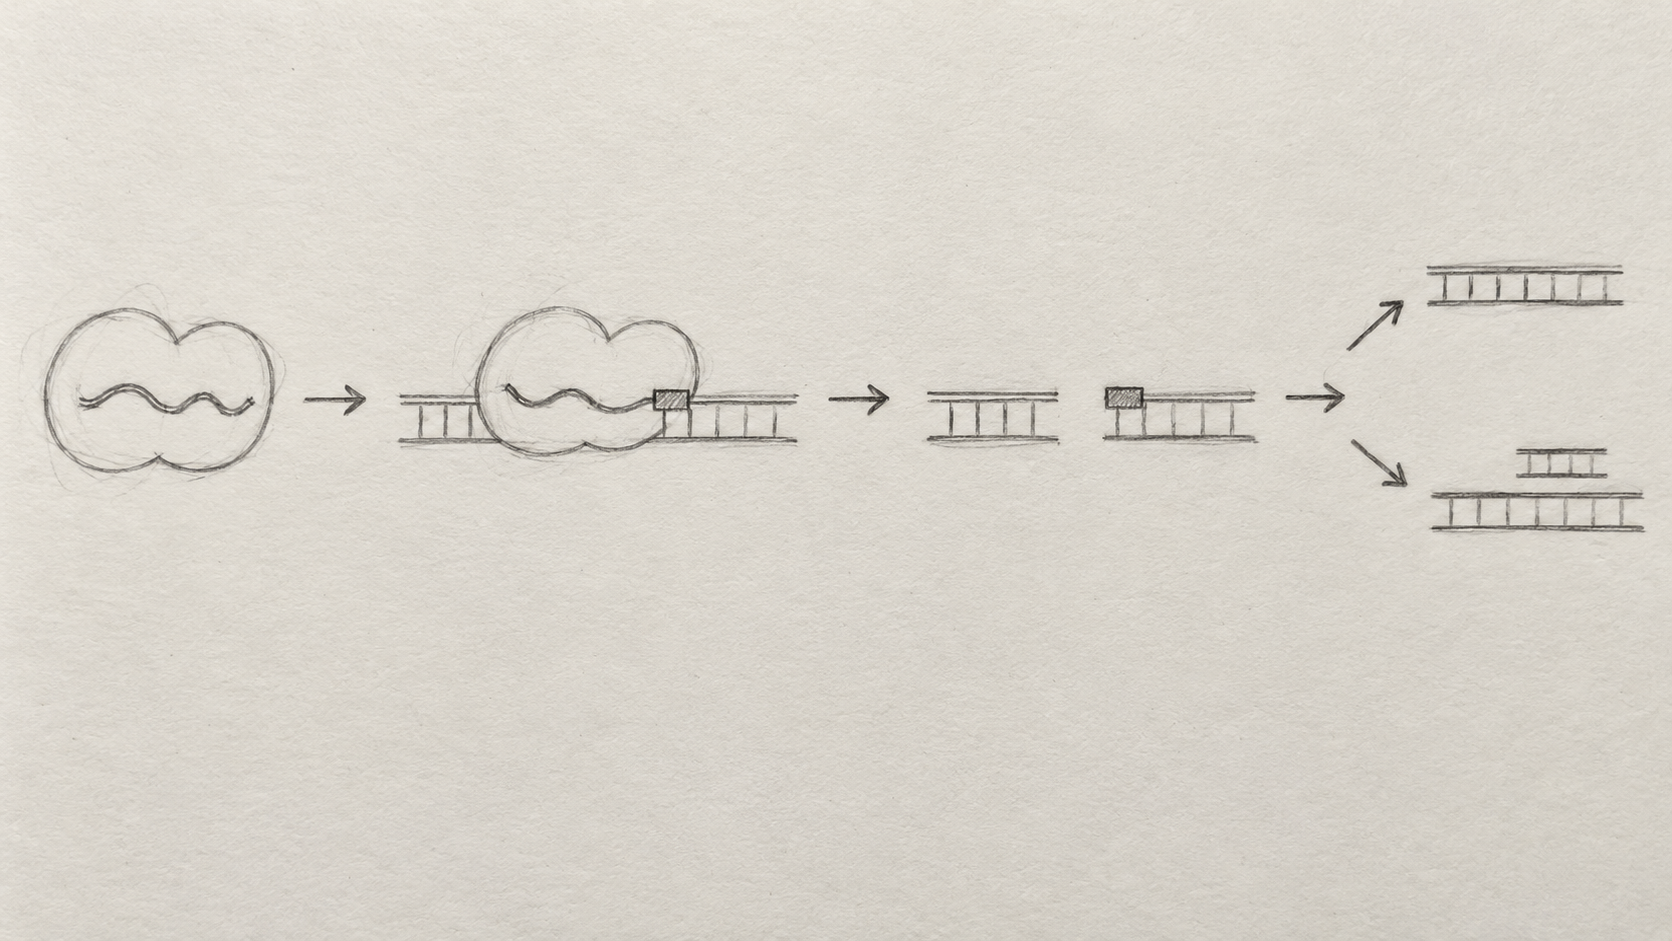
\includegraphics[width=\linewidth]{figures/ch03/ch03-02a-sketch-linear.png}};
\begin{scope}[x={(img.south east)},y={(img.north west)}]
  \node[font=\sffamily\bfseries\normalsize, anchor=north west, text=BookInk] at (0.04,0.94) {A};
\end{scope}
\end{tikzpicture}\\[1mm]
{\footnotesize A\quad 线性（左$\rightarrow$右）}
\end{minipage}\hfill
\begin{minipage}[t]{0.32\linewidth}\centering
\begin{tikzpicture}
\node[anchor=south west,inner sep=0] (img) at (0,0) {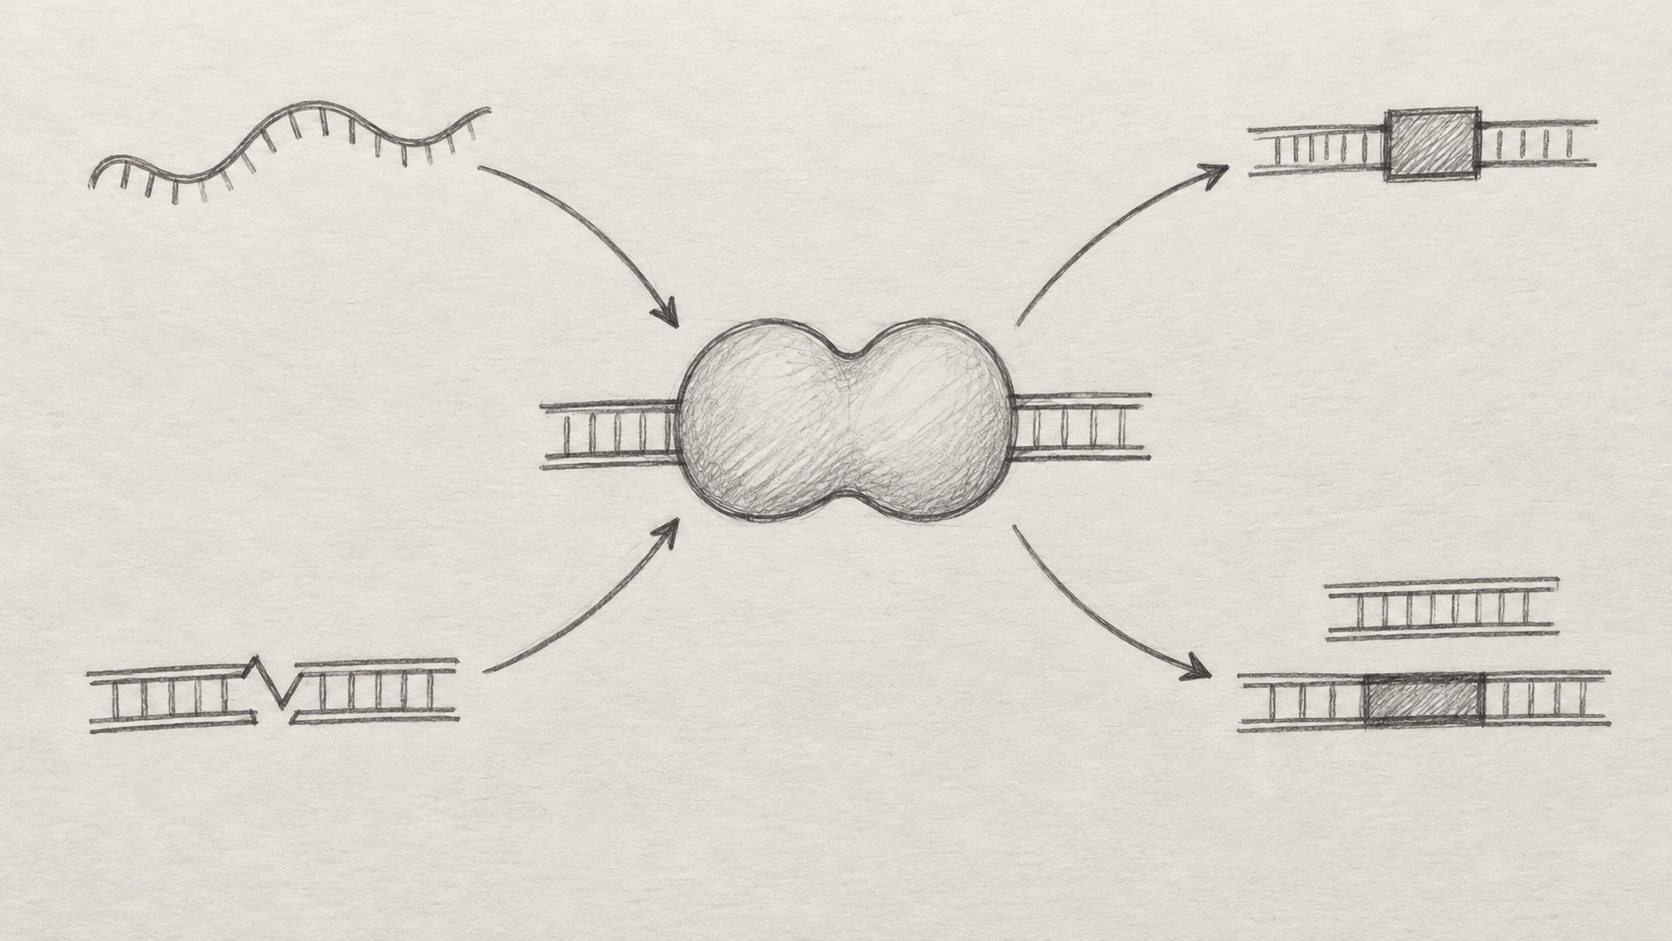
\includegraphics[width=\linewidth]{figures/ch03/ch03-02b-sketch-hub.png}};
\begin{scope}[x={(img.south east)},y={(img.north west)}]
  \node[font=\sffamily\bfseries\normalsize, anchor=north west, text=BookInk] at (0.04,0.94) {B};
\end{scope}
\end{tikzpicture}\\[1mm]
{\footnotesize B\quad 中心辐射}
\end{minipage}\hfill
\begin{minipage}[t]{0.32\linewidth}\centering
\begin{tikzpicture}
\node[anchor=south west,inner sep=0] (img) at (0,0) {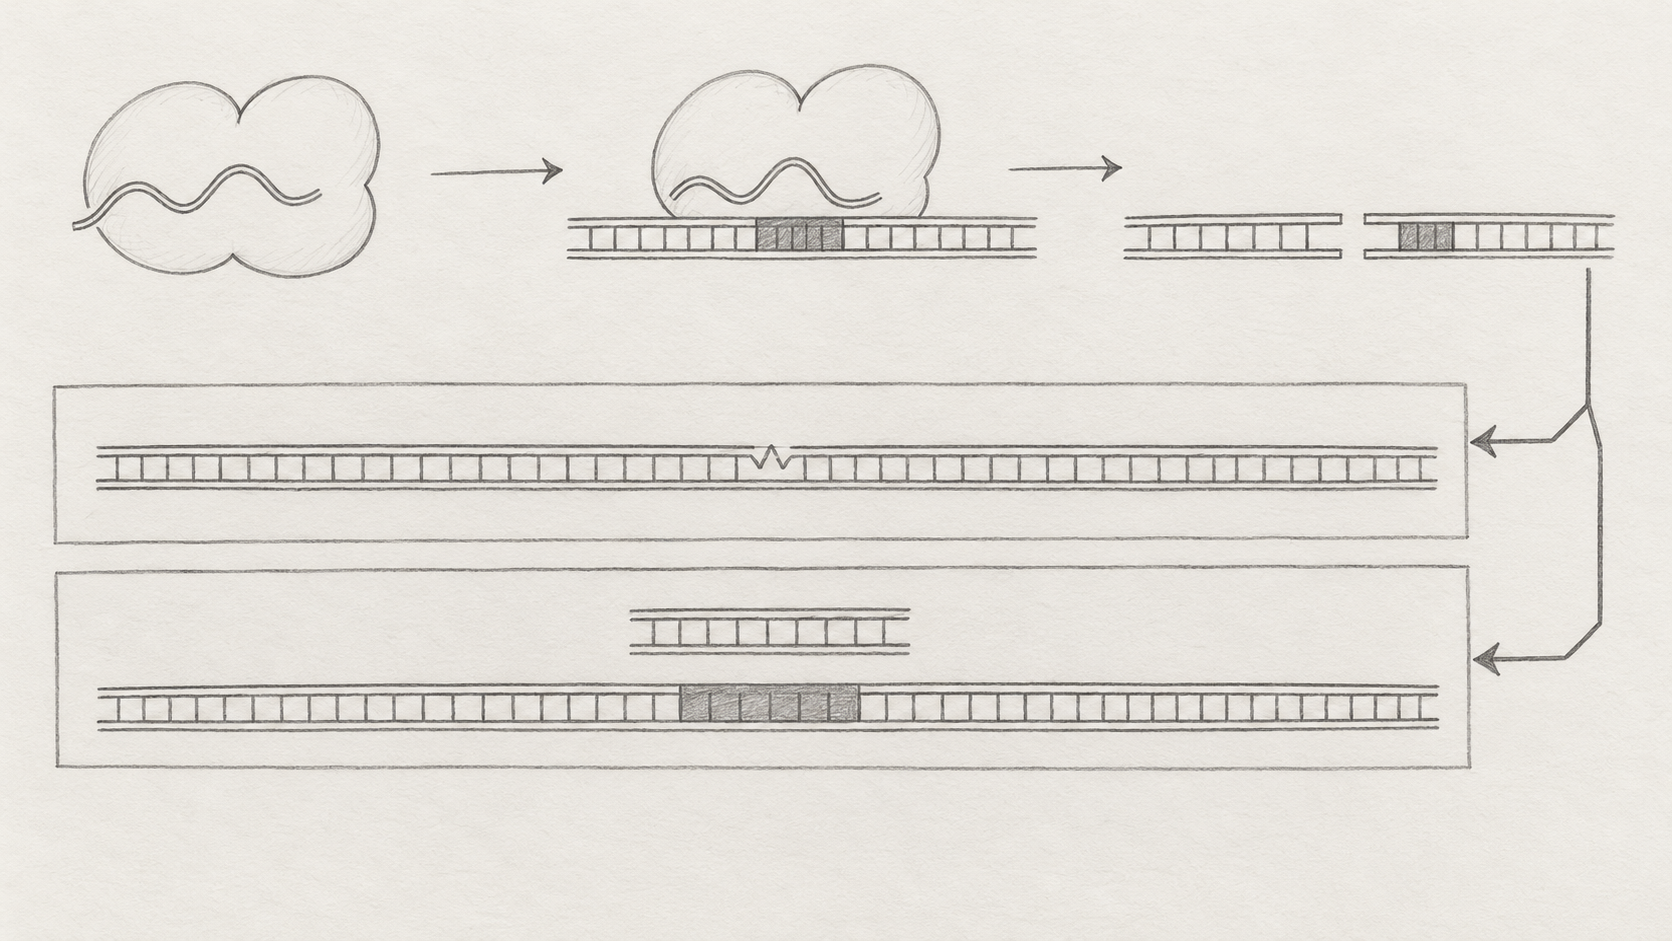
\includegraphics[width=\linewidth]{figures/ch03/ch03-02c-sketch-branch.png}};
\begin{scope}[x={(img.south east)},y={(img.north west)}]
  \node[font=\sffamily\bfseries\normalsize, anchor=north west, text=BookInk] at (0.04,0.94) {C};
\end{scope}
\end{tikzpicture}\\[1mm]
{\footnotesize C\quad 两分支结果}
\end{minipage}
\caption{同一内容的三种草图骨架（图像模型模拟的铅笔草图）。草图只确定分区、相对大小、箭头方向与留白，不写文字；对象的含义由任务书规定。A 把事件排成一行；B 以 Cas9–DNA 复合物为中心；C 把前三步压缩在上排，下方并列两条修复通道。本章示例图由图像模型生成，提示词与生成记录见本书仓库。}\label{fig:ch03-02}
\end{figure}

观察图~\ref{fig:ch03-02} 的生成过程与实际画面，可以总结出三点直接有用的经验：

第一，\textbf{线性单行最容易一次成形，但右端对比区天然局促。} 图~\ref{fig:ch03-02}A 第一次生成就排出了从左到右的四个阶段与右端分叉（阶段间以短箭头指示方向），但因前三步占去了左起大半宽度，右端上下叠放的两条结果双链被挤压得很短。

第二，\textbf{中心辐射结构天然抹平事件起点。} 生成图~\ref{fig:ch03-02}B 时，第一次抽样曾把左下角的 indel 折线画成了脱离 DNA 的大闪电，且箭头从右上、右下指向中心；第二次抽样恢复了贴附在双链上的小折线，四支单头箭头呈“左上与左下指向中心、中心指向右上与右下”的两进两出格局（中央蛋白铅笔排线较重），画面没有唯一入口。

第三，\textbf{模型对“分叉进入两个不同通道”的拓扑路由非常迟钝。} 生成图~\ref{fig:ch03-02}C 时，前两次抽样虽然画出了上排三步和下方两个铅笔矩形框，但模型连续两次把从第三步向下分叉出来的\textbf{两个箭头全部指在了上方通道框的上沿}，导致下方通道没有入口箭头，且上通道 DNA 中间裂成了大缺口。直到第三次抽样专门补充路由说明——要求分叉干线沿右侧框外下行，一支从右端进入上框，另一支继续向下从右端进入下框，且上框 DNA 保持连续只在中部画小折线——才得到图~\ref{fig:ch03-02}C 的正确连接。即便如此，仔细检查图~\ref{fig:ch03-02}C 仍可见上下两个铅笔框高度并不完全相等（下框略高），且左上蛋白内的 RNA 呈双描线。这说明作者自己拿铅笔在纸上花一分钟画出分叉箭头和等高通道，比纯靠文字让模型猜拓扑要高效得多。

送入下一步前，用四项标准自检每张草图：是否一眼能看出入口；分叉点是否清楚且两条结果画成并列；留白是否足够放标签；画面是否无文字。

\section{从草图到候选图，再到选择}

接着在 \scidraw{} 提示词绘图（\sdtool{ai-drawing}）中切换到\textbf{草图模式}，分别上传三张草图，粘贴同一份由任务书转化的英文提示词生成三张候选图。三次生成只替换上传的草图与末尾对应的布局句，而把视觉风格、对象颜色身份、步骤定义与禁止项保持一致，这样比较才公平。完整英文提示词分两段给出如下：

\begin{Prompt}
Flat 2D scientific overview schematic for a journal figure, landscape 16:9, pure white background. Clean vector illustration style: flat fills, thin dark gray outlines, no gradients, no shadows, no highlights, no 3D, no glow, no texture. ABSOLUTELY NO TEXT: no letters, no words, no numbers, no symbols, no labels, no legend, no title.
Follow the layout of the attached pencil sketch closely: same regions, same relative positions, same arrow directions.
OBJECTS (use these exact visual identities in every step where they appear):
- Cas9: a rounded two-lobed protein shape, muted blue-gray (#7C93A8).
- sgRNA: a single orange (#E69F00) strand with a short straight segment (the spacer) and a small hairpin loop scaffold, partly inside Cas9.
- Genomic DNA: two parallel dark gray (#4D4D4D) lines with short light gray rungs between them.
- PAM: a short bright yellow (#F0E442) segment on the upper DNA line.
- Double-strand break: a clean gap through both DNA lines, right next to the PAM.
- Donor template: a short separate double-stranded DNA; its two ends dark gray (homology arms), its middle segment teal (#009E73).
- NHEJ result: a continuous DNA with one small reddish-purple (#CC79A7) mark at the former break site.
- HDR result: a continuous DNA with a teal (#009E73) segment at the former break site, the same length as the donor's middle segment.
\end{Prompt}

\begin{Prompt}
STEPS: (1) Cas9 bound to sgRNA. (2) Cas9-sgRNA sitting on the DNA at the PAM, the orange spacer lying alongside the lower DNA line, the upper line slightly pushed away. (3) The DNA with the break next to the PAM, Cas9 lifted away. (4) Repair by end joining, giving the NHEJ result, with no donor. (5) Repair using the donor template, giving the HDR result; the donor appears only here. Steps are connected by solid dark gray arrows with filled heads; after step 3 the arrow splits into two equal arrows.
DO NOT DRAW: cells, nucleus, chromosomes, scissors, lightning, sparkles, double-helix twisting, realistic protein structure, any charts or data. Bottom 10% of the image empty.
LAYOUT [A]: one row of five steps left to right; steps 4 and 5 stacked at the right end.
LAYOUT [B]: radial; the DNA-bound Cas9 complex (step 2-3 merged) in the center, steps 1, 4, 5 and the PAM detail around it.
LAYOUT [C]: steps 1-3 as a compact row across the top third; below, two equal-height horizontal lanes stacked vertically, upper lane step 4, lower lane step 5, with the DNA in both lanes aligned at the same x positions and length.
\end{Prompt}

使用草图模式时必须明确一条边界：\textbf{草图是布局意图的强提示，而不是像素级布局锁定。} 模型在把铅笔草图渲染成彩色图形时，仍可能发生对象位置漂移、复制或身份互换。因此生成后必须先将候选图与原草图并排核对，再叠加阅读顺序编号（图~\ref{fig:ch03-03}）。

\begin{figure}[htbp]\centering
\begin{minipage}[t]{0.32\linewidth}\centering
\begin{tikzpicture}[ord/.style={circle, draw=orange!85!black, line width=0.6pt, fill=orange!15, inner sep=1pt, font=\sffamily\bfseries\scriptsize, text=BookInk}]
\node[anchor=south west,inner sep=0] (img) at (0,0) {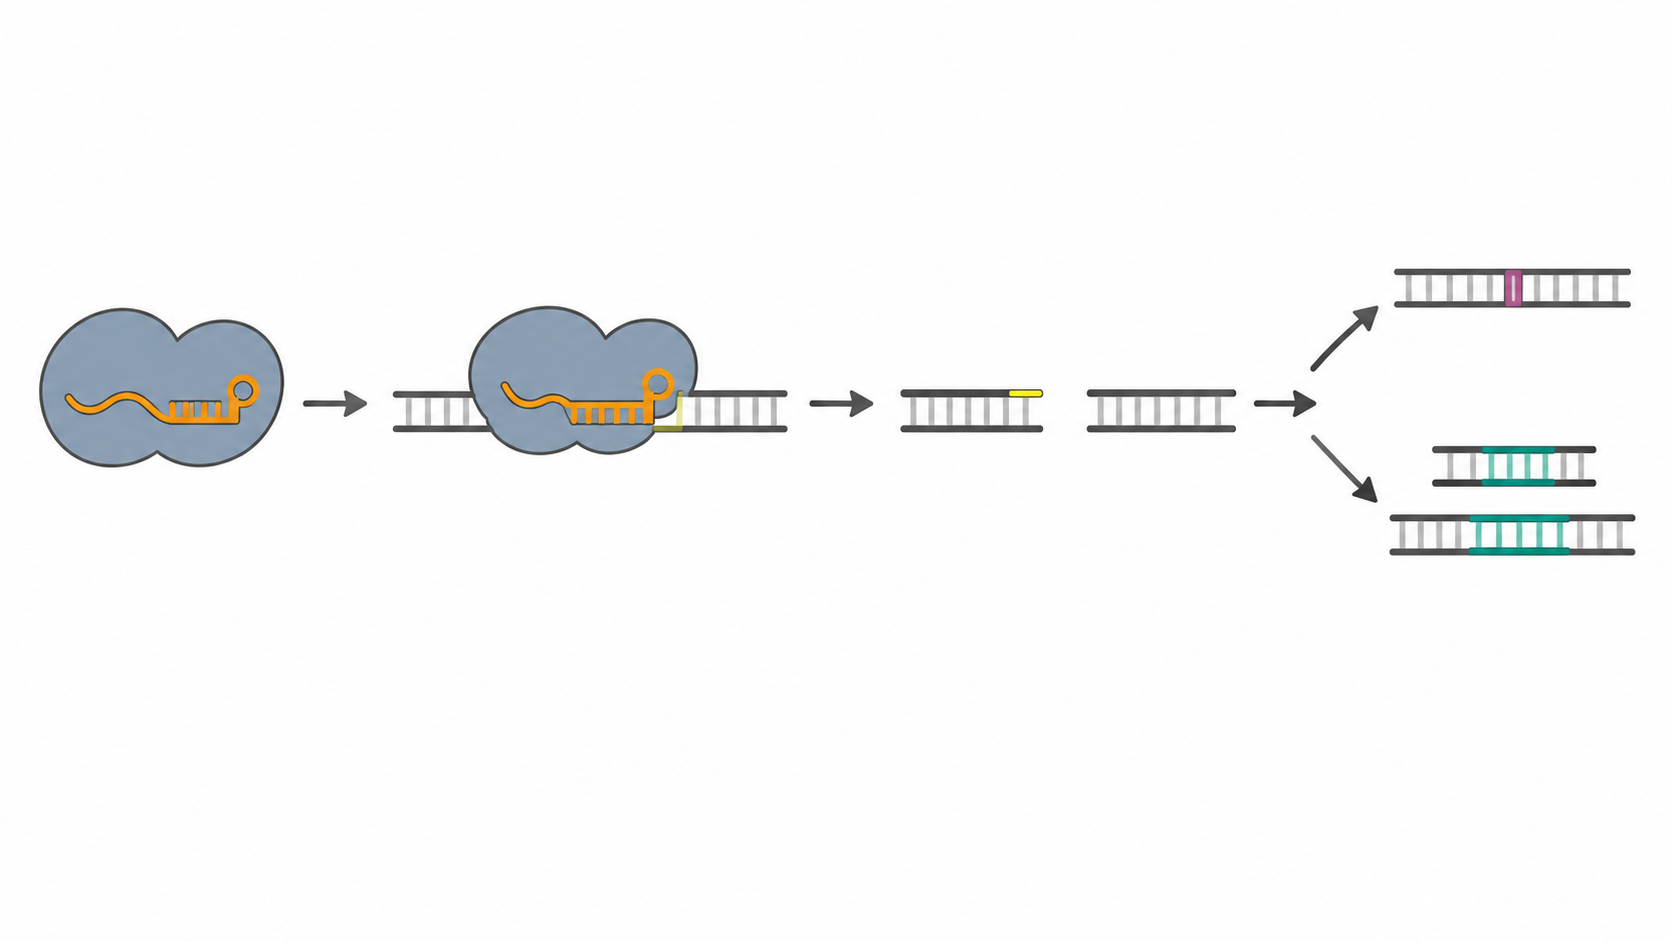
\includegraphics[width=\linewidth]{figures/ch03/ch03-03a-cand-linear.png}};
\begin{scope}[x={(img.south east)},y={(img.north west)}]
  \node[font=\sffamily\bfseries\normalsize, anchor=north west, text=BookInk] at (0.04,0.94) {A};
  \node[ord] at (0.08,0.55) {1};
  \node[ord] at (0.27,0.55) {2};
  \node[ord] at (0.46,0.55) {3};
  \node[ord] at (0.80,0.72) {4};
  \node[ord] at (0.80,0.35) {5};
\end{scope}
\end{tikzpicture}
\end{minipage}\hfill
\begin{minipage}[t]{0.32\linewidth}\centering
\begin{tikzpicture}[ord/.style={circle, draw=orange!85!black, line width=0.6pt, fill=orange!15, inner sep=1pt, font=\sffamily\bfseries\scriptsize, text=BookInk}]
\node[anchor=south west,inner sep=0] (img) at (0,0) {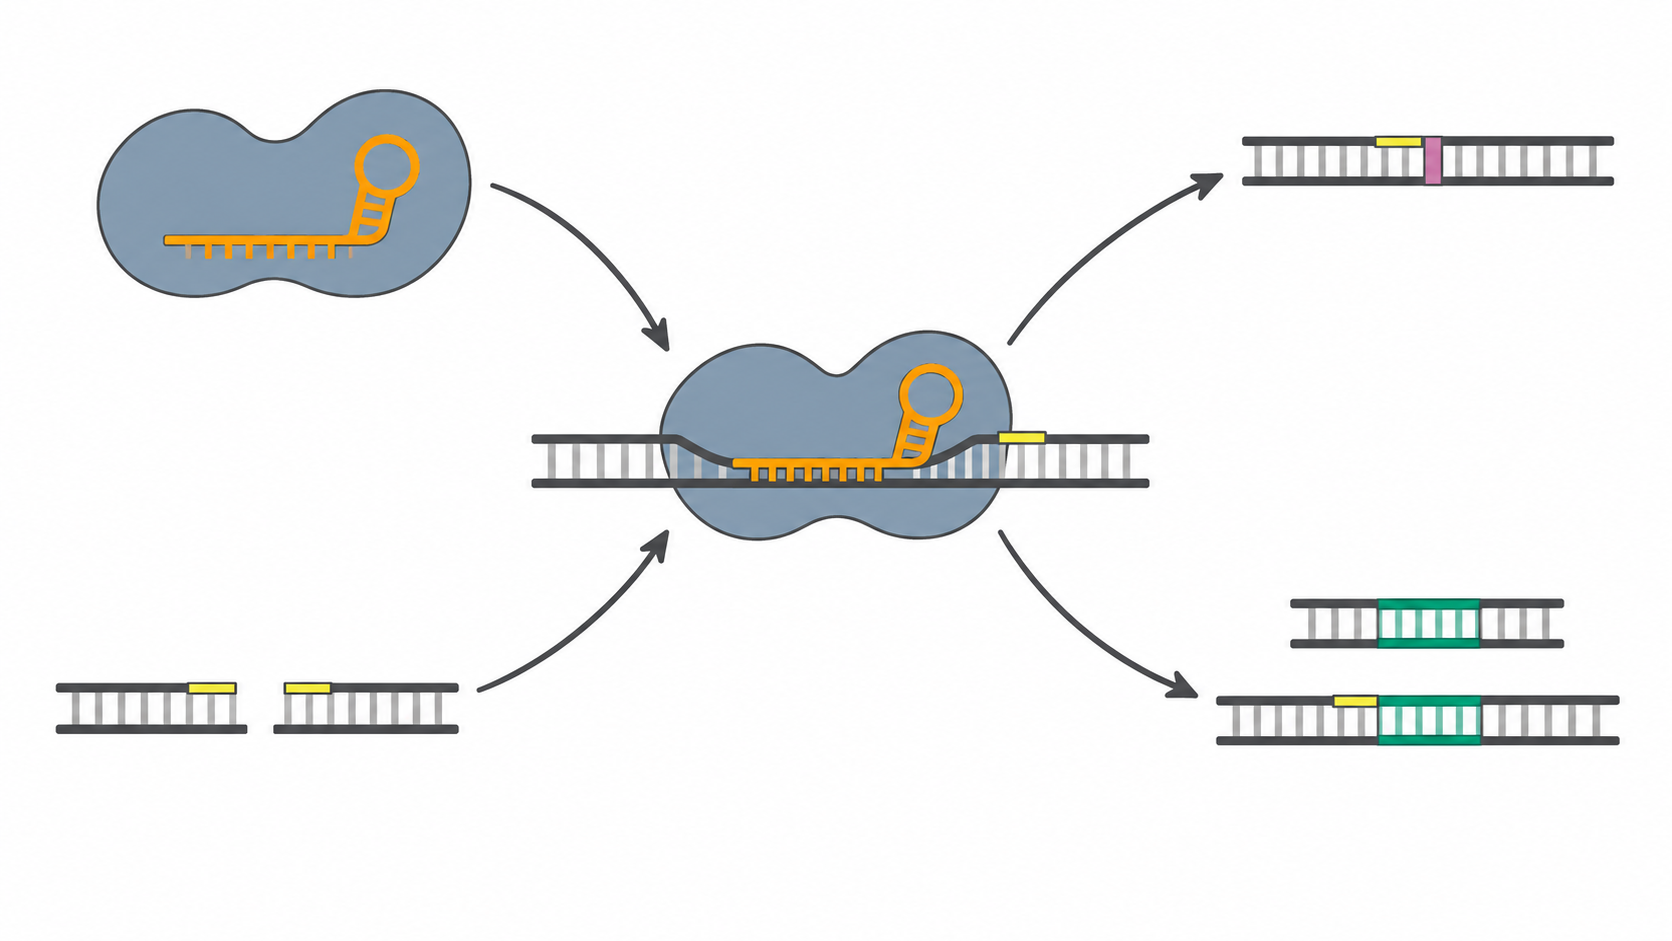
\includegraphics[width=\linewidth]{figures/ch03/ch03-03b-cand-hub.png}};
\begin{scope}[x={(img.south east)},y={(img.north west)}]
  \node[font=\sffamily\bfseries\normalsize, anchor=north west, text=BookInk] at (0.04,0.94) {B};
  \node[ord] at (0.50,0.52) {1?};
\end{scope}
\end{tikzpicture}
\end{minipage}\hfill
\begin{minipage}[t]{0.32\linewidth}\centering
\begin{tikzpicture}[ord/.style={circle, draw=orange!85!black, line width=0.6pt, fill=orange!15, inner sep=1pt, font=\sffamily\bfseries\scriptsize, text=BookInk}]
\node[anchor=south west,inner sep=0] (img) at (0,0) {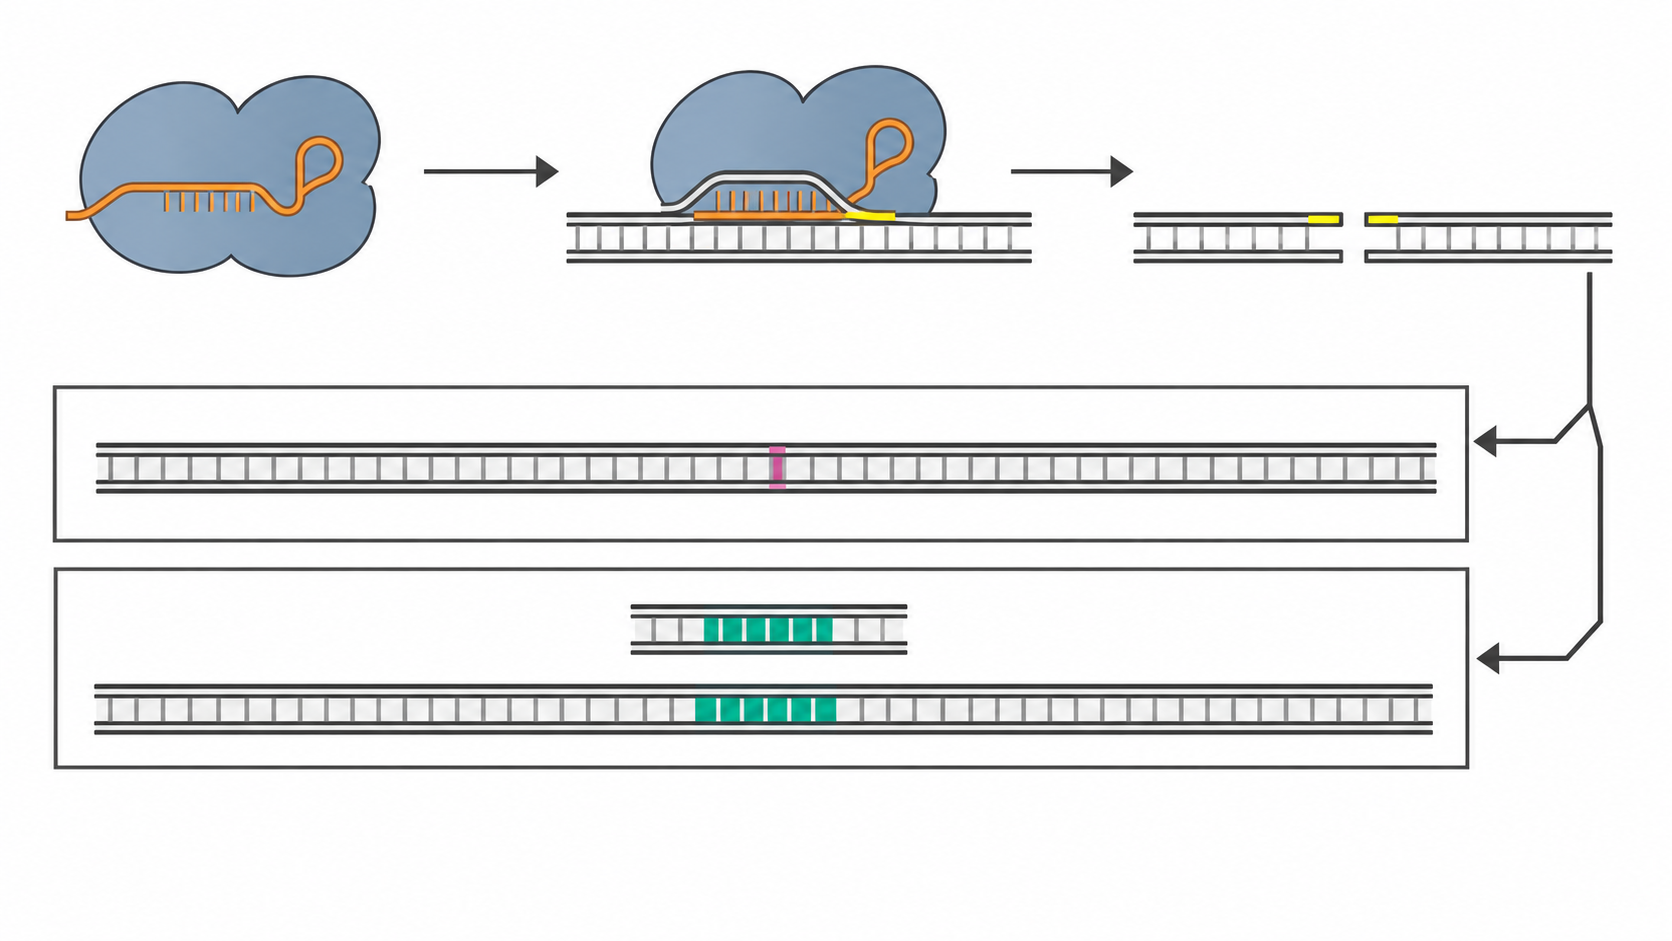
\includegraphics[width=\linewidth]{figures/ch03/ch03-03c-cand-branch.png}};
\begin{scope}[x={(img.south east)},y={(img.north west)}]
  \node[font=\sffamily\bfseries\normalsize, anchor=north west, text=BookInk] at (0.04,0.94) {C};
  \node[ord] at (0.15,0.85) {1};
  \node[ord] at (0.38,0.85) {2};
  \node[ord] at (0.62,0.85) {3};
  \node[ord] at (0.50,0.55) {4};
  \node[ord] at (0.50,0.22) {5};
\end{scope}
\end{tikzpicture}
\end{minipage}
\caption{同一份任务书、三张不同草图得到的候选图。橙色编号标出作者预期的阅读顺序（实际课题中应请未看过任务书的同事独立测试编号）：A 与 C 的顺序清晰且与事件先后一致；B 中左上与左下两支箭头同时指向中心，缺少唯一入口。生成后已对照草图核查位置偏离。}\label{fig:ch03-03}
\end{figure}

逐张对照图~\ref{fig:ch03-02} 与图~\ref{fig:ch03-03} 的实际画面，我们可以清楚看到三种骨架的表现及位置偏离：

\begin{itemize}
\item \textbf{候选 A（线性，图~\ref{fig:ch03-03}A）：} 一次生成即遵循了草图 A 从左到右的单行排布，Cas9（蓝灰）、sgRNA（橙）、DNA（深灰）、PAM（亮黄）、indel（红紫）及供体与写入段（青绿）的颜色角色全部准确，供体仅出现在右下角。但对照草图 A 检查第三步（切割步骤）时，发现了一处典型的**位置漂移**：草图 A 中位于缺口**右侧**的 PAM 阴影块，在候选 A 中被模型移到了缺口**左侧**；同时第二步 R 环配对关系不够清晰，最右端上下叠放的两个结果区域十分拥挤，供体中段与写入段的青绿长度也未严格相等。
\item \textbf{候选 B（中心辐射，图~\ref{fig:ch03-03}B）：} 这张图生动证明了“不良布局骨架会连带诱发科学内容错误”。前两次生成时，模型先后擅自把左下箭头反转为向外（把左上变成伪入口，并将单条 sgRNA 扩画成完整 Cas9–sgRNA 复合物）或画成双向箭头；第三次补充“严格保留左上、左下向内，右上、右下向外四支单头箭头”的说明后，虽然箭头方向对上了草图，画面却发生了严重的**对象身份交换与标记增殖**：原本在草图左下角的 NHEJ 结果（红紫标记）跑到右上角去了，左下角变成了断裂 DNA；而且左下缺口左右两侧、右上红紫标记左侧及右下青绿写入段左侧全都多出了一段黄色 PAM，正中央复合物处反而看不出双链断裂。同时，把“sgRNA”“断裂 DNA”与“修复结果”画成围绕中心的同级卫星节点，彻底拉平了事件层级。
\item \textbf{候选 C（两分支，图~\ref{fig:ch03-03}C）：} 一次生成即完整保留了“上排紧凑三步 + 右侧分叉 + 下方上下并列双通道”的骨架，短双链供体准确地只出现在下方 HDR 通道内且居中于青绿写入段上方，两条结果长 DNA 的左右端点也高度对齐（水平误差不到链长的 0.3\%），未出现细胞核等排除对象。但放大检查仍能定位两处待改问题：第一，上排第三步双链断裂的\textbf{缺口左右两侧各出现了一段黄色 PAM}（重复画了两个 PAM）；第二，下方两个矩形通道框高度明显不等，下框比上框高出约 29\%（此外三张候选图的蛋白与橙线均带轻微明暗高光，未做到绝对平涂）。
\end{itemize}

在实际课题中，此时应把三张无编号的候选图拿给一至两位没看过任务书的同事，请他们凭直觉标出阅读顺序 1–5（也可以请能看图的对话式 AI 描述它会先看哪里作为辅助参考，但不能替代真人测试）。接着，用一张写明客观标准的比较表（表~\ref{tab:ch03-02-cmp} 与图~\ref{fig:ch03-04}）作出选择，而不是凭“哪张更顺眼”。

\begin{table}[htbp]\centering\footnotesize
\setlength{\tabcolsep}{3pt}
\renewcommand{\arraystretch}{1.15}
\caption{三种布局候选方案的比较表。}\label{tab:ch03-02-cmp}
\begin{tabularx}{\linewidth}{@{}>{\raggedright\arraybackslash}p{36mm}YYY@{}}
\toprule
\textbf{标准} & \textbf{A 线性} & \textbf{B 中心辐射} & \textbf{C 两分支} \\
\midrule
入口是否唯一明确 & 是（左端步骤 1） & 否（左上与左下两进两出） & 是（左上角步骤 1） \\
阅读方向与事件先后一致 & 是 & 部分（需完全靠箭头，且对象错位） & 是 \\
两种结果能否在同一基线上直接对照 & 否（上下挤在右端） & 否（分散在右上与右下角） & 是（上下并列宽通道，端点对齐） \\
主要信息（同一断裂、两种结果）的视觉权重 & 低（占右端约 11\%--25\%） & 中（分散在角落，约 25\%） & 高（占下半幅约 50\%） \\
174 mm 宽下的标签空间 & 紧 & 中 & 足 \\
适合的用途 & 幻灯片逐步展示 & 概念关系图（非时序） & 论文总览图 \\
\bottomrule
\end{tabularx}
\end{table}

\begin{figure}[htbp]\centering
\resizebox{\linewidth}{!}{% FIG ch03-04 layout comparison (Chinese)
\begin{tikzpicture}[
  x=1mm, y=1mm,
  font=\sffamily\footnotesize,
  text=BookInk,
  wf/.style={draw=black!50, fill=black!4, line width=0.4pt},
  main/.style={fill=teal!25, draw=none},
]
  \def\fw{52}\def\fh{33}
  \begin{scope}[shift={(0,58)}]
    \draw[wf] (0,0) rectangle (\fw,\fh);
    \fill[main] (0.68*\fw,0.05*\fh) rectangle (0.96*\fw,0.43*\fh);
    \node[anchor=north, font=\bfseries] at (0.5*\fw,\fh+2) {A};
    \node[font=\scriptsize, anchor=south] at (0.5*\fw,-1.5) {约 11\%};
  \end{scope}
  \begin{scope}[shift={(56,58)}]
    \draw[wf] (0,0) rectangle (\fw,\fh);
    \fill[main] (0.15*\fw,0.12*\fh) rectangle (0.85*\fw,0.47*\fh);
    \node[anchor=north, font=\bfseries] at (0.5*\fw,\fh+2) {B};
    \node[font=\scriptsize, anchor=south] at (0.5*\fw,-1.5) {约 25\%};
  \end{scope}
  \begin{scope}[shift={(112,58)}]
    \draw[wf] (0,0) rectangle (\fw,\fh);
    \fill[main] (0,0) rectangle (\fw,0.50*\fh);
    \node[anchor=north, font=\bfseries] at (0.5*\fw,\fh+2) {C};
    \node[font=\scriptsize, anchor=south] at (0.5*\fw,-1.5) {约 50\%};
  \end{scope}
  \node[font=\scriptsize, text=BookInk!70, anchor=north west] at (0,54)
    {青绿区为两种修复结果所占面积（线框示意；候选 PNG 实测后更新）};

  \matrix (m) [
    matrix of nodes,
    anchor=north west,
    row sep=1.8mm,
    column sep=3mm,
    nodes={font=\scriptsize, inner sep=2pt},
    column 1/.style={nodes={anchor=west}, text width=38mm},
    column 2/.style={nodes={anchor=center}, text width=12mm},
    column 3/.style={nodes={anchor=center}, text width=12mm},
    column 4/.style={nodes={anchor=center}, text width=12mm},
  ] at (0,48) {
    & {A} & {B} & {C} \\
    入口唯一 & {$\bullet$} & {$\circ$} & {$\bullet$} \\
    顺序与事件一致 & {$\bullet$} & {\tikz[baseline=-0.6ex]{\fill[BookTeal] (0,0) arc (90:270:0.35); \draw[BookTeal] (0,0) circle (0.35);}} & {$\bullet$} \\
    两种结果可直接对照 & {$\circ$} & {$\circ$} & {$\bullet$} \\
    主要信息的面积 & {$\circ$} & {\tikz[baseline=-0.6ex]{\fill[BookTeal] (0,0) arc (90:270:0.35); \draw[BookTeal] (0,0) circle (0.35);}} & {$\bullet$} \\
    174\,mm 下标签空间 & {\tikz[baseline=-0.6ex]{\fill[BookTeal] (0,0) arc (90:270:0.35); \draw[BookTeal] (0,0) circle (0.35);}} & {\tikz[baseline=-0.6ex]{\fill[BookTeal] (0,0) arc (90:270:0.35); \draw[BookTeal] (0,0) circle (0.35);}} & {$\bullet$} \\
    适合的用途 & {幻灯片} & {概念图} & {论文总览} \\
  };
  \draw[BookTeal, line width=0.8pt, rounded corners=1pt]
    ([xshift=-2mm,yshift=2mm]m-1-4.north west) rectangle ([xshift=2mm,yshift=-2mm]m-7-4.south east);
\end{tikzpicture}
}
\caption{按写明的标准比较三种布局。上：线框中青绿区域为“两种修复结果”所占版面面积比例示意。下：逐项判定矩阵。选择 C 作为论文总览图；A 保留用于汇报幻灯片的逐步呈现。}\label{fig:ch03-04}
\end{figure}

如图~\ref{fig:ch03-04} 所示，本图的主要信息是“同一断裂、两种修复结果”，布局 C 将下半幅约 50\% 的版面完整分配给两条对齐的修复通道，读者能在同一水平位置直接比较 indel 与精确写入。因此我们在修改记录中写明选择理由：\textbf{选定 C 作为论文总览图；保留 A 用于汇报幻灯片的逐步动画版本；淘汰 B。}

\section{每次只改一个可核对的目标}

以候选 C 为起点进入修改阶段时，切忌下达“把细节改对、通道对齐、画面更简洁”的混合指令。参考图修改（在 \scidraw{} 中选中历史图并输入修改指令）本质上是条件重绘而非矢量软件的局部平移；如果一条指令里塞进三四个目标，不仅容易顾此失彼，而且一旦出现新错误，你根本无法判断是哪句话触发了模型的误操作。

正确的修订纪律是：\textbf{每次只提出一个可核对的目标，采用“具体改动目标 + 保持不变的内容 + 检查方法”的格式，并在每次修改后与上一版叠图对比，如实填写意外变化日志。}

我们先在候选 C（图~\ref{fig:ch03-05} 左）上对四个预设核查点（编号 1 至 4）做定点诊断，区分真问题与已达标项：

\begin{itemize}
\item \textbf{核查点 1（PAM 位置）：} 上排右侧切割步骤的缺口左右两侧各有一段黄色 PAM，左侧那段属于重复错误，\textbf{必须擦除左侧黄段、只保留右侧上链紧邻缺口的 PAM}。
\item \textbf{核查点 2（供体模板位置）：} 事先担心供体漂在通道之间或出现两次；实测候选 C 中短双链供体已经唯一地位于下方 HDR 通道内且大致居中。为检验单目标微调并使其青绿中段与写入段严格居中对齐，我们仍执行一次微调指令。
\item \textbf{核查点 3（两条通道对齐）：} 实测下方两条长 DNA 的左右端点水平误差已小于 0.3\%（满足 $<2\%$ 的要求），但\textbf{两个矩形通道外框的高度相差约 29\%}（下框明显高于上框），需要把两框高度调齐。
\item \textbf{核查点 4（多余背景对象）：} 事先准备了第 4 条指令用于删除可能出现的细胞核轮廓或装饰背景；实测候选 C 背景干净、无任何多余对象，因此\textbf{第 4 条修改指令直接跳过不执行}。
\end{itemize}

四条预设单目标修改指令的英文原文如下：

\begin{Prompt}
[Revision 1 - PAM position] Edit the selected image. Change only one thing: move the small yellow PAM segment so that it sits directly next to the right side of the DNA gap at the cleavage step, on the upper strand, touching the gap. Keep every other object, color, line weight and position unchanged. Do not add any text.
\end{Prompt}

\begin{Prompt}
[Revision 2 - Donor placement] Edit the selected image. Change only one thing: move the short teal donor DNA so that it lies inside the lower repair lane only, directly above the DNA gap in that lane, horizontally centered on the gap. Remove any copy of the donor outside the lower lane. Keep everything else unchanged. No text.
\end{Prompt}

\begin{Prompt}
[Revision 3 - Lane alignment] Edit the selected image. Change only one thing: make the two repair lanes the same height, and draw the DNA in both lanes at the same horizontal position and the same length, so the two results line up vertically for comparison. Keep colors, objects and the top row unchanged. No text.
\end{Prompt}

\begin{Prompt}
[Revision 4 - Remove extra objects, conditional] Edit the selected image. Remove the cell nucleus outline and any background shapes. Change nothing else. No text.
\end{Prompt}

\begin{figure}[htbp]\centering
\begin{minipage}[t]{0.49\linewidth}\centering
\begin{tikzpicture}[font=\sffamily\footnotesize, text=BookInk]
  \node[inner sep=0, anchor=south west] (imga) at (0,0) {%
    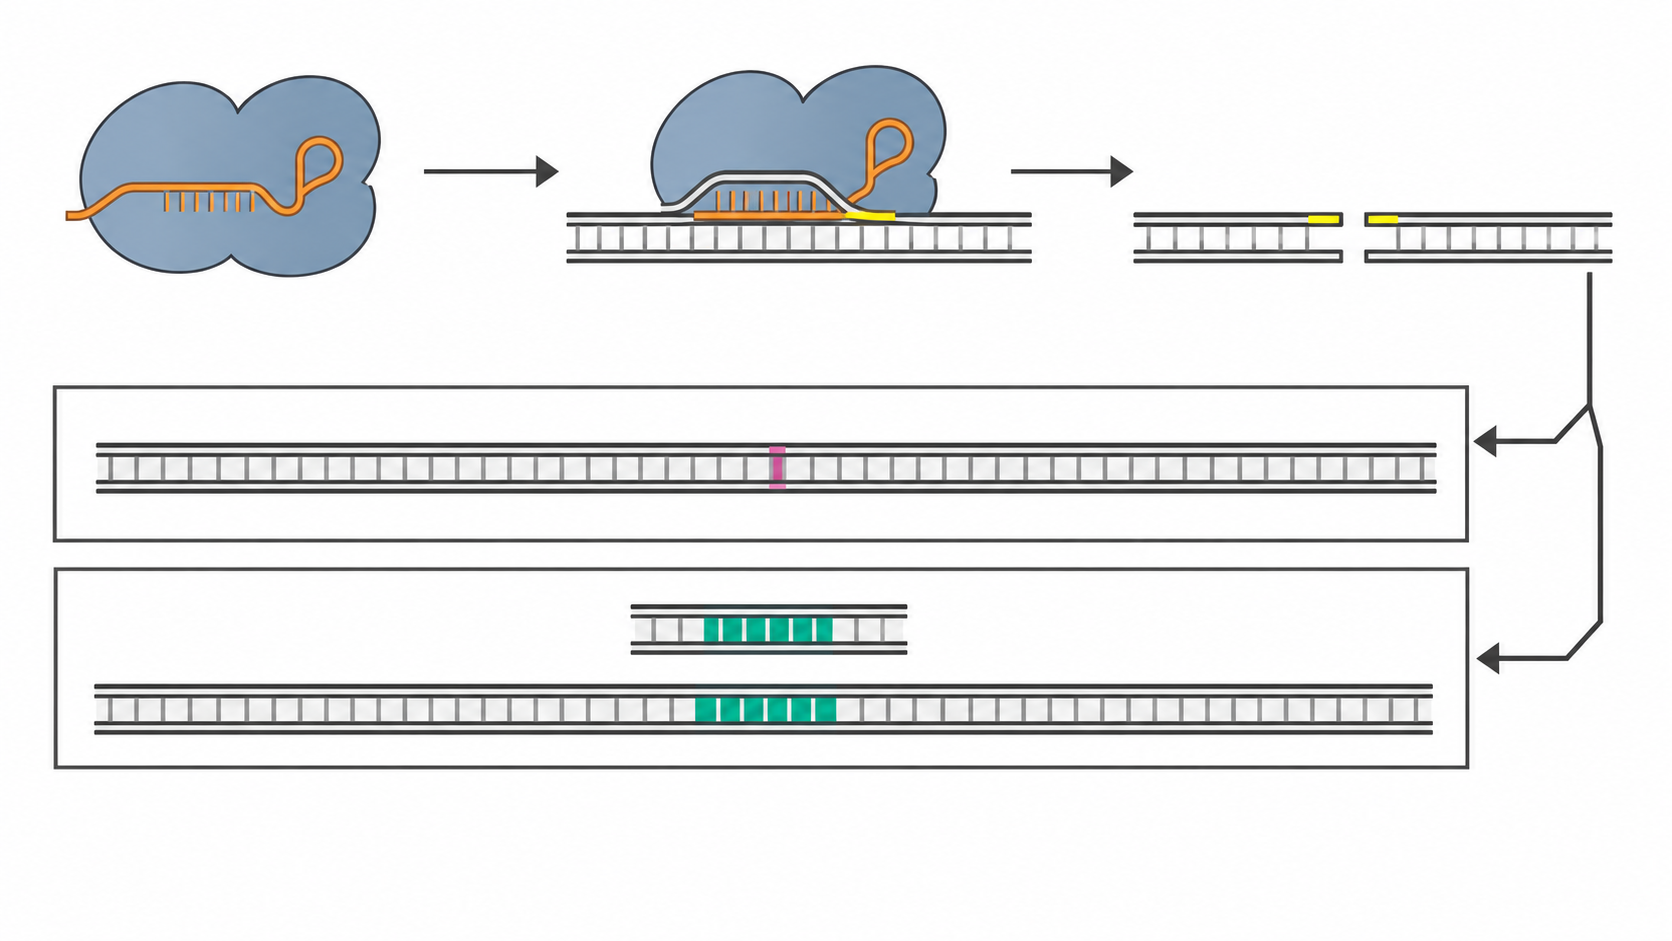
\includegraphics[width=\linewidth]{figures/ch03/ch03-03c-cand-branch.png}};
  \begin{scope}[x={(imga.south east)},y={(imga.north west)},
    issuemark/.style={circle, draw=red!75!black, line width=0.6pt, fill=white, fill opacity=0.88, text opacity=1, inner sep=0.8pt, font=\sffamily\bfseries\scriptsize, text=red!75!black}]
    \node[issuemark] at (0.62,0.78) {1};
    \node[issuemark] at (0.48,0.42) {2};
    \node[issuemark] at (0.72,0.28) {3};
    \node[issuemark] at (0.88,0.65) {4};
    \node[anchor=west, align=left, font=\sffamily\scriptsize] at (0.02,0.08) {%
      1 PAM 位置\quad 2 供体模板位置\\
      3 通道未对齐\quad 4 多余对象排查};
  \end{scope}
\end{tikzpicture}
\end{minipage}\hfill
\begin{minipage}[t]{0.49\linewidth}\centering
\begin{tikzpicture}[font=\sffamily\footnotesize, text=BookInk]
  \node[inner sep=0, anchor=south west] (imgb) at (0,0) {%
    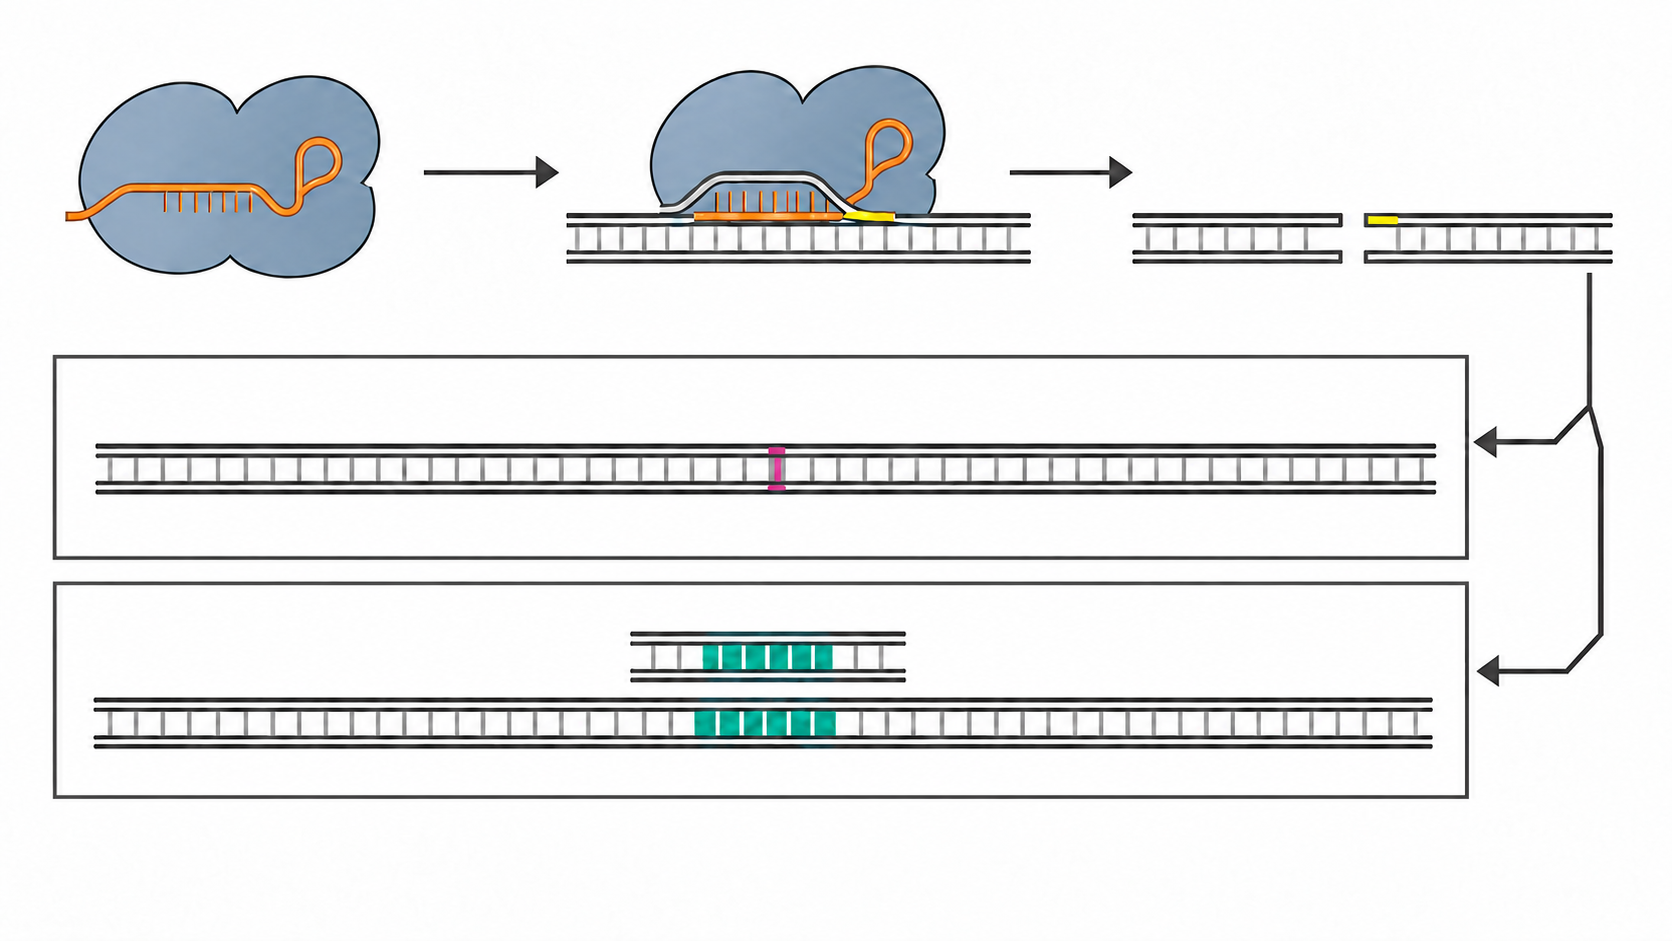
\includegraphics[width=\linewidth]{figures/ch03/ch03-05b-v3-revised.png}};
  \begin{scope}[x={(imgb.south east)},y={(imgb.north west)}]
    \draw[green!55!black, line width=0.8pt] (0.14,0.80) circle (0.07);
    \draw[green!55!black, line width=0.8pt] (0.48,0.29) circle (0.09);
    \node[anchor=west, align=left, font=\sffamily\scriptsize, text=green!45!black] at (0.02,0.08) {%
      意外变化：sgRNA 高光重绘、\\
      下通道微移及残留约 6\% 框高差};
  \end{scope}
\end{tikzpicture}
\end{minipage}
\caption{逐条修改。左：候选 C 的四个核查点，其中 1 处切口两侧重复画出黄色 PAM，3 处两通道外框高度明显不等（2 处供体已在下通道内，4 处实测无多余背景对象）。右：依次执行单目标修改后的版本；切口左侧重复 PAM 已消除，两框高度差大幅缩小；绿色圆圈标出未要求却发生的轻微重绘与位移，已记入修改记录。}\label{fig:ch03-05}
\end{figure}

表~\ref{tab:ch03-03-log} 完整记录了从候选 C 到图~\ref{fig:ch03-05} 右的七次真实调用与意外变化处理过程：

\begin{table}[htbp]\centering\footnotesize
\setlength{\tabcolsep}{3pt}
\renewcommand{\arraystretch}{1.15}
\caption{从候选 C 到修订稿的意外变化日志。}\label{tab:ch03-03-log}
\begin{tabularx}{\linewidth}{@{}>{\raggedright\arraybackslash}p{24mm}ccY>{\raggedright\arraybackslash}p{20mm}@{}}
\toprule
\textbf{修改阶段} & \textbf{尝试} & \textbf{达成} & \textbf{未要求却发生的变化（及是否影响科学）} & \textbf{处理决定} \\
\midrule
修改 1：PAM 位置 & 1 & 否 & 切口两侧仍有两个黄色 PAM；细线轻微再渲染（不影响科学） & 退回候选 C \\
修改 1：补充定位 & 2 & \textbf{是} & 左侧重复 PAM 消除；细描边与色彩纹理轻微再渲染（无影响） & \textbf{保留}为基准 1 \\
修改 2：供体居中 & 1 & 否 & \textbf{下通道内唯一的短双链供体被直接删掉（影响科学）} & \textbf{弃用}，退回基准 1 \\
修改 2：保护供体 & 2 & \textbf{是} & 供体保留并与青绿段对齐；供体整体下移约 15 像素（无影响） & \textbf{保留}为基准 2 \\
修改 3：通道等高 & 1 & 部分 & \textbf{供体消失；两条结果 DNA 均出现红紫和青绿（影响科学）} & \textbf{弃用}，退回基准 2 \\
修改 3：保护身份 & 2 & 否 & 科学身份恢复，但下框被进一步拉高、下通道下移（几何未达标） & 弃用，退回基准 2 \\
修改 3：抬高上框 & 3 & \textbf{是} & 框高差由 29.4\% 降至 6.0\%，端点误差 0.22\%；下通道微移、sgRNA 高光微变（无影响） & \textbf{保留}为修订稿 \\
修改 4：删背景 & 0 & — & 画面无细胞核或多余背景形状 & 条件跳过 \\
\bottomrule
\end{tabularx}
\end{table}

从表~\ref{tab:ch03-03-log} 的真实记录中，可以提炼出三条直接指导日常作图的修改准则：

\textbf{第一，当原指令首次调用无效时，补充“当前哪里错了、擦除什么、保留什么”的具体定位。} 修改 1 第 1 次调用之所以无效，是因为切口右侧本来就有一段黄色 PAM，模型认为要求已满足而保留了左侧多余黄段；第 2 次明确补充“擦除缺口左侧黄色高亮并恢复为深灰 DNA 线、仅保留右侧上链紧贴缺口的一段黄色高亮”，立即一次奏效。

\textbf{第二，警惕局部修改引发“误删唯一对象”或“抹平对照差异”的严重副作用，一旦发生立即回退上一版。} 修改 2 第 1 次调用时，模型过度响应“Remove any copy”，竟把下通道里唯一的短双链供体删光了；修改 3 第 1 次调用时，模型过度响应“same height and length”，不仅删掉供体，还把上下两条结果 DNA 都画成了同时带红紫和青绿的混合体，直接毁掉了 NHEJ 与 HDR 的科学对照！遇到这种破坏科学内容的意外变化，绝不能在坏图上继续发指令打补丁，而必须\textbf{立即退回上一轮验证通过的基准版}，在指令中补上保护性约束（如“上通道只保留红紫 indel、无青绿无供体；下通道保留青绿写入段及上方唯一短供体，仅抬高上框顶边”）重新生成。

\textbf{第三，区分“科学硬伤”与“无害的渲染波动”，适时停手或切换确定性工具。} 图~\ref{fig:ch03-05} 右侧绿色细圈标出了三轮修改积累的轻微连带变化：上排 sgRNA 橙色高光与轮廓粗细微变、下通道整体微幅下移，且两框仍留有约 6.0\% 的高度差（较最初的 29.4\% 已大幅改善，长 DNA 左右端点误差仅 0.22\%）。由于这些变化完全不影响 C1–C9 的科学含义与视觉比对，将其记入日志后即可接受定稿。反之，若同一局部指令重试 3 次仍不断破坏其他关键对象，则应停止生成式修改，把精确几何交给 TikZ 绘制。

\section{案例收束：终稿、图注与核验}

为了在总览图右上角嵌入图~\ref{fig:ch03-07} 的确定性 PAM 细节插图，我们以图~\ref{fig:ch03-05} 右为参考图，执行最后一次版面留白调整，将上排三步向左紧凑移动，腾出右上角约 30\% 宽度的空白：

\begin{Prompt}
Edit the selected image. Change only one thing: shift the three steps of the top row to the left so that the right 30% of the top row is empty white space. Keep sizes, colors and the two lower lanes unchanged. No text.
\end{Prompt}

这一步同样经过三次抽样筛选：第 1 次右上仅腾出约 23\% 宽度且第三步与右侧分叉干线脱节；第 3 次虽留白充足，但模型把第三步连接线改为只指向 NHEJ 上框，与右侧双分支干线断开，破坏了“同一断裂分出两条途径”的路径拓扑；因此最终选定\textbf{第 2 次抽样}作为终稿无字底图——上排三步紧凑左移（伴随未要求的轻微缩小），折线从第三步顺畅接入右侧共同分叉干线，右上角腾出约 30\% 宽、约 32\% 高的无遮挡区域（仅底缘有一段水平连接线经过）。灰度检查表明，亮黄色 PAM（带深色描边）与青绿色供体存在显著明度对比，黑白打印下仍可清晰区分。

随后在 LaTeX/TikZ 中采用 book-spec 规范的相对坐标叠加写法，将图~\ref{fig:ch03-07} 缩放嵌入右上角空白区，并叠加全部中文矢量标签、步骤编号 1–5 与底部图例，合成终稿（图~\ref{fig:ch03-06}）。

\begin{figure}[htbp]\centering
\begin{tikzpicture}[font=\sffamily\scriptsize, text=BookInk]
  \node[anchor=south west, inner sep=0] (img) at (0,0) {%
    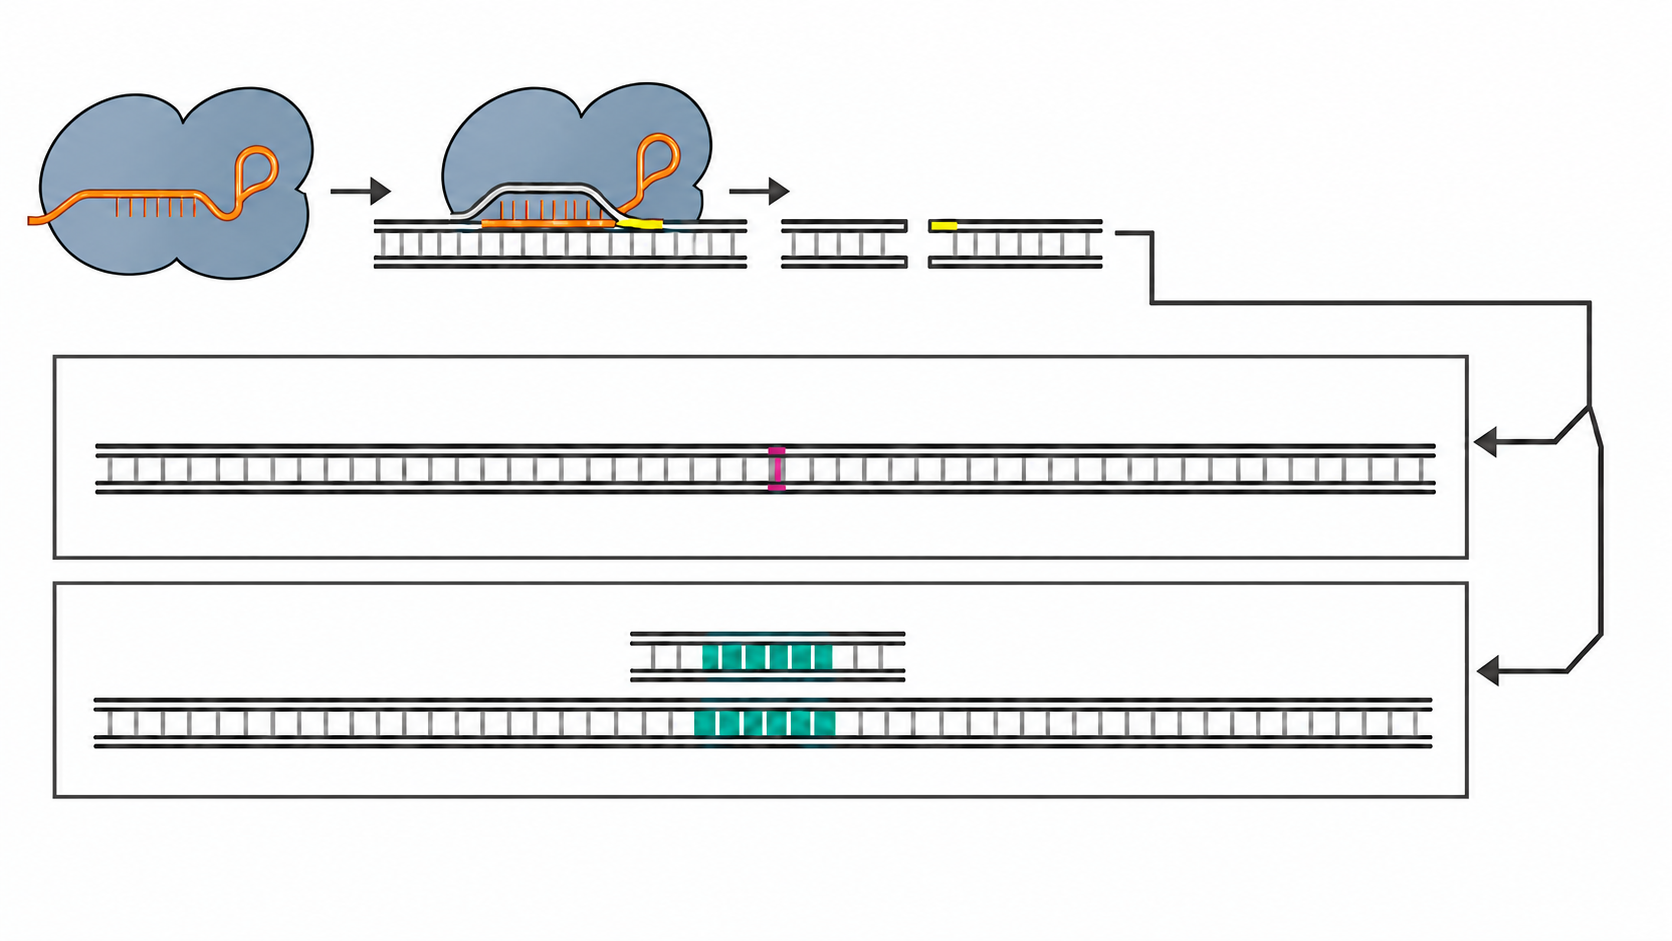
\includegraphics[width=\linewidth]{figures/ch03/ch03-06-final-base.png}};
  \begin{scope}[x={(img.south east)}, y={(img.north west)},
    lbl/.style={font=\sffamily\scriptsize, fill=white, fill opacity=0.88, text opacity=1, inner sep=1pt},
    ord/.style={circle, draw=orange!85!black, line width=0.5pt, fill=orange!15, inner sep=0.8pt, font=\sffamily\bfseries\tiny, text=BookInk}]
    \node[anchor=south west, inner sep=0, fill=white, fill opacity=0.92, text opacity=1] at (0.64,0.60) {%
      \resizebox{0.35\linewidth}{!}{% FIG ch03-07 PAM inset (Chinese)
\begin{tikzpicture}[
  x=1mm, y=1mm,
  font=\sffamily\scriptsize,
  text=BookInk,
]
  \node[anchor=east] at (-2, 21.2) {非靶链};
  \node[anchor=east] at (-2, 7.2) {靶链};
  \node at (6, 23.6) {5$'$};
  \node at (54.5, 23.6) {3$'$};
  \node at (55.5, 4.4) {5$'$};
  \node at (6, 4.4) {3$'$};

  \foreach \i in {0,...,19} {
    \pgfmathsetmacro{\x}{6+\i*2.4}
    \draw[draw=BookInk!50, fill=white] (\x,20) rectangle (\x+2.4,22.4);
  }
  \foreach \i in {0,1,2} {
    \pgfmathsetmacro{\x}{6+(17+\i)*2.4}
    \draw[draw=BookInk!50, fill=yellow!70] (\x,20) rectangle (\x+2.4,22.4);
  }
  \node[anchor=west, text=BookInk!80] at (6+17*2.4, 28.2) {PAM（NGG）};

  \foreach \i in {0,...,19} {
    \pgfmathsetmacro{\x}{6+\i*2.4}
    \draw[draw=BookInk!50, fill=white] (\x,6) rectangle (\x+2.4,8.4);
  }
  \foreach \i in {0,...,19} {
    \pgfmathsetmacro{\x}{6+\i*2.4}
    \draw[BookInk!35, thin] (\x+1.2,8.4) -- (\x+1.2,11.6);
    \draw[draw=orange!80!black, fill=orange!25, line width=1pt]
      (\x,4) rectangle (\x+2.4,6.4);
  }
  \draw[orange!80!black, line width=0.8pt]
    (6+19*2.4+2.4, 5) .. controls (6+21*2.4, 8) .. (6+21*2.4, 12)
    .. controls (6+21*2.4, 14) .. (6+19*2.4, 14);

  \node[anchor=west] at (6, 0.5) {sgRNA 间隔序列};
  \pgfmathsetmacro{\cx}{6+16.5*2.4+1.2}
  \fill[black] (\cx,20) -- (\cx-0.8,21.2) -- (\cx+0.8,21.2) -- cycle;
  \fill[black] (\cx,6) -- (\cx-0.8,4.8) -- (\cx+0.8,4.8) -- cycle;
  \node[anchor=west] at (6+17.5*2.4, 13) {切点};
  \node[anchor=west, font=\scriptsize] at (6+16*2.4, 17) {RuvC};
  \node[anchor=west, font=\scriptsize] at (6+16*2.4, 3) {HNH};

  \draw[decorate, decoration={brace, amplitude=3pt}] (6, 15.5) -- (6+20*2.4, 15.5)
    node[midway, above=4pt] {约 20 nt};
  \draw[decorate, decoration={brace, amplitude=2pt, mirror}] (6+16*2.4, 22.5) -- (6+17*2.4, 22.5)
    node[midway, below=2pt] {3 bp};
\end{tikzpicture}
}};
    \node[ord] at (0.04,0.92) {1};
    \node[ord] at (0.24,0.92) {2};
    \node[ord] at (0.46,0.82) {3};
    \node[ord] at (0.03,0.52) {4};
    \node[ord] at (0.03,0.22) {5};
    \node[lbl, font=\sffamily\bfseries\scriptsize] at (0.10,0.92) {Cas9};
    \node[lbl, font=\sffamily\bfseries\scriptsize] at (0.06,0.72) {sgRNA};
    \node[lbl] at (0.38,0.70) {PAM};
    \node[lbl] at (0.30,0.62) {靶 DNA};
    \node[lbl] at (0.52,0.62) {双链断裂};
    \node[lbl, anchor=west] at (0.06,0.48) {NHEJ（无模板）};
    \node[lbl, anchor=west] at (0.06,0.22) {HDR（供体模板）};
    \node[lbl] at (0.55,0.40) {小片段插入/缺失};
    \node[lbl] at (0.50,0.34) {供体模板};
    \node[lbl] at (0.55,0.12) {精确编辑};
    \node[font=\sffamily\scriptsize, align=left, anchor=north west] at (0.02,0.05) {%
      图例：实线箭头 = 步骤；分叉箭头 = 两种可选修复途径；黄色 = PAM；红紫 = indel；青绿 = 供体来源序列};
  \end{scope}
\end{tikzpicture}
\caption{CRISPR–Cas9 基因组编辑总览图终稿。无字底图叠加矢量标签、底部图例与右上角确定性 PAM 细节插图（图~\ref{fig:ch03-07}）。完整中英文图注见正文。}\label{fig:ch03-06}
\end{figure}

编写图注时，若使用 \scidraw{} 的图注辅助工具（\sdtool{figure-legend}）起草初稿，作者必须逐句核实简化声明与文献依据，严禁编造任何效率数值、样本量（\texttt{n=}）或统计显著性结论。完整的中英文图注如下：

\begin{BookNote}
\textbf{图 1　CRISPR–Cas9 基因组编辑及两种主要修复结果示意。} 单链引导 RNA（sgRNA）与 Cas9 结合；复合物识别基因组 DNA 上的 PAM（SpCas9 为 $5'$-NGG-$3'$），sgRNA 的约 20 nt 间隔序列与靶链配对，Cas9 在 PAM 上游约 3 bp 处切开两条链，形成双链断裂。断裂可经非同源末端连接（NHEJ）修复，该途径不需要模板，可能在断裂处留下小片段插入或缺失（indel），位于编码区时可能破坏基因功能；在提供带同源臂的供体模板时，也可经同源定向修复（HDR）按模板写入精确改变，HDR 在多数细胞中频率低于 NHEJ。插图示意 PAM、靶链、非靶链与切点的相对位置。为便于阅读，图中省略了 Cas9 的三维结构与 HNH/RuvC 结构域的分工（插图除外）、修复途径的分子因子、替代末端连接途径、脱靶切割及递送方式。依据 Jinek 等（2012）、Doudna 与 Charpentier（2014）、Hsu 等（2014）整理。

\medskip
\textbf{Figure 1 | Overview of CRISPR–Cas9 genome editing and its two main repair outcomes.} A single guide RNA (sgRNA) binds Cas9. The complex recognizes a protospacer-adjacent motif (PAM; $5'$-NGG-$3'$ for SpCas9) in genomic DNA, the $\sim$20-nt spacer of the sgRNA base-pairs with the target strand, and Cas9 cleaves both strands about 3 bp upstream of the PAM, creating a double-strand break. The break can be repaired by non-homologous end joining (NHEJ), which needs no template and may leave small insertions or deletions (indels) that can disrupt a coding sequence; when a donor template with homology arms is supplied, homology-directed repair (HDR) can instead copy a precise change from the template. In most cell types HDR is less frequent than NHEJ. The inset shows the positions of the PAM, the target and non-target strands and the cleavage site. For clarity, the three-dimensional structure of Cas9, the division of labour between the HNH and RuvC domains (except in the inset), repair factors, alternative end-joining pathways, off-target cleavage and delivery methods are omitted. Based on Jinek et al.\ (2012), Doudna and Charpentier (2014) and Hsu et al.\ (2014).
\end{BookNote}

最后，对照关系表 C1–C9 对终稿图~\ref{fig:ch03-06} 做逐条核验（表~\ref{tab:ch03-04-verify}）。

\begin{table}[htbp]\centering\footnotesize
\setlength{\tabcolsep}{3pt}
\renewcommand{\arraystretch}{1.15}
\caption{CRISPR–Cas9 总览图终稿核验记录表。}\label{tab:ch03-04-verify}
\begin{tabularx}{\linewidth}{@{}l>{\raggedright\arraybackslash}p{22mm}>{\raggedright\arraybackslash}p{34mm}cY@{}}
\toprule
\textbf{\#} & \textbf{关系} & \textbf{图中应见} & \textbf{结论} & \textbf{备注} \\
\midrule
C1 & sgRNA–Cas9 结合 & 步骤 1 两者接触成复合物 & $\checkmark$ & 橙色 sgRNA 与蓝灰 Cas9 接触，发夹可辨 \\
C2 & 识别 PAM & 步骤 2 复合物停在黄色 PAM 处 & $\checkmark$ & 复合物邻近亮黄色 PAM 段 \\
C3 & 间隔序列与靶链配对 & RNA 与一条 DNA 链平行贴合，另一条被推开 & 部分 & 底图有置换拱起但横档使配对链身份略含混；由右上角确定性插图精确阐明 \\
C4 & PAM 位置 & 黄色段在非靶链、紧邻配对区一端（插图精确） & $\checkmark$ & 底图切口右侧上链保留单一黄段；右上插图精确锁定非靶链 $3'$ 侧 $5'$-NGG-$3'$ \\
C5 & 双链断裂 & 两条链在同一处断开，紧邻 PAM & $\checkmark$ & 底图双链同处断开；上游约 3 bp 距离及 HNH/RuvC 分工由右上插图表达 \\
C6/C7 & NHEJ 结果 & 无模板；断裂处有红紫 indel 标记 & $\checkmark$ & 上通道 4 无模板，中部带单一红紫标记；图注写明“可能” \\
C8/C9 & HDR 结果 & 供体只在此通道；结果 DNA 含青绿写入段 & 部分 & 下通道 5 含唯一短供体及正下方青绿写入段（两段青绿长度接近，属示意表达） \\
— & 阅读顺序 & 1–5 编号路径与预期一致 & $\checkmark$ & 上排 1–3 接右侧分叉入 4–5；长 DNA 端点误差 0.22\%（正式提交前补同事盲测） \\
— & 禁止项 & 无细胞核、剪刀、发光、底图文字 & $\checkmark$ & 200\% 放大检查底图无文字及违禁对象 \\
— & 复核 & 由做基因编辑的同行签名复核 & 待完成 & 投稿前请基因编辑方向同行复核插图链方向、HNH/RuvC 标注与图注措辞 \\
\bottomrule
\end{tabularx}
\end{table}

回顾全过程，本案例归档的交付物涵盖：三张草图、三张候选图及偏离记录、比较表与选择理由、单目标修改指令与意外变化日志、确定性插图、无字底图与合成终稿、中英文图注及核验记录表。

\section{AI 在这一步能做什么与不能做什么}

构图推演与草图迭代环节中 AI 与作者的职责边界汇总于表~\ref{tab:ch03-01}。

\begin{table}[htbp]\centering\footnotesize
\setlength{\tabcolsep}{3pt}
\renewcommand{\arraystretch}{1.15}
\caption{AI 在构图与草图环节能做什么、不能做什么及作者要核对的内容。}\label{tab:ch03-01}
\begin{tabularx}{\linewidth}{@{}>{\raggedright\arraybackslash}p{20mm}YYY@{}}
\toprule
\textbf{环节} & \textbf{AI 能做} & \textbf{AI 不能做 / 不可靠} & \textbf{作者要核对} \\
\midrule
提出布局骨架 & 对话式 AI 可按任务书用文字列出几种布局思路及其阅读顺序 & 不会自动根据论文判断哪种布局最好；\scidraw{} 的批量候选共享同一提示词，结构差异有限，不会独立规划不同方案并解释理由 & 至少有一个骨架是自己画的；三种骨架在结构上真的不同 \\
草图 $\rightarrow$ 候选图 & \scidraw{} 草图模式可把草图与提示词一起作为输入，较快得到遵循大致布局的候选图 & 草图不等于布局锁定：对象可能漂移、合并、缺失、新增或互换身份 & 对照草图逐项检查位置、方向、数量；记录偏离 \\
阅读顺序评估 & 可请能看图的对话式 AI 描述“它会先看哪里”，作为一个额外视角 & 模型的描述不等于真实读者的视线；不能代替同行测试 & 至少请一位没看过任务书的人编号；以人的结果为准 \\
选择布局 & 可帮助把比较标准整理成表格 & 不能替作者决定什么是主要信息 & 主要信息写在任务书里；选择理由写进修改记录 \\
修改 & 参考图修改可按指令调整位置、删除对象、改外框或颜色 & 局部指令可能引起连带变化；同一指令结果不稳定；无法精确控制几何关系（链方向、碱基距离） & 每次一个目标；与上一版叠图比较；填写意外变化日志；精确几何改用 TikZ \\
科学正确性 & 能按给定关系画出示意 & 不会自己发现 PAM 画错链、切点离 PAM 太远、供体或颜色标记混淆 & 按关系表 C1–C9 逐条核验；领域同行复核 \\
文字与标签 & —（底图要求无文字） & 生成图中的文字常拼错、错位 & 标签在 LaTeX/TikZ 中叠加，作者校对拼写与位置 \\
\bottomrule
\end{tabularx}
\end{table}

\section{本章检查清单}

\begin{itemize}
\item 我能用一句话说出这张图的入口、路径和终点。
\item 图中只有一个视觉最重的元素，而且它承载主要信息。
\item 放在同一组（接近、对齐、围合）的对象确实相关；无关对象没有被意外分到一组。
\item 分叉处两条路径画成并列选项，读者不会误以为是先后步骤。
\item 需要精确几何关系的细节（链方向、位置、距离）用确定性工具绘制，或单独成插图。
\item 我画了至少三种结构不同的草图，并保存了它们。
\item 生成候选图时，每次只换草图、不换任务书核心文字。
\item 我对照草图记录了每张候选图的位置偏离。
\item 阅读顺序由至少一位没看过任务书的人测试过。
\item 选择理由写成了可核对的标准，而不是“更好看”。
\item 每条修改指令只有一个目标，并写明保持不变的内容。
\item 每次修改后都填写了意外变化日志，并保存了中间版本。
\item 终稿底图无文字，标签与图例在 LaTeX 中叠加，按最终尺寸检查了字号。
\end{itemize}

\section{练习}

\begin{enumerate}
\item \textbf{（纸笔：给一张图找入口）} 从你所在领域近期的一篇论文中选一张总览图或图形摘要。（a）不看图注，用 5 秒看图，写下你看到的第一、第二、第三个元素；（b）再请一位同学独立做同样的事；（c）比较两人的顺序，指出是哪些手段（尺寸、对比、位置、箭头、编号）造成了一致或分歧；（d）在复印件上画出你认为更好的视线路径，并说明需要移动哪两个元素。
\item \textbf{（\scidraw{} 实操：一份任务书，三张草图）} 选择一个包含“分叉”或“对比”的过程（例如：一种材料的两种失效模式，一项算法的两种分支处理）。（a）写出关系表和任务书；（b）手绘线性、中心辐射、分支对比三张草图并拍照；（c）在 \scidraw{} 草图模式中，用同一份任务书文字分别上传三张草图生成候选图；（d）对照草图记录每张的偏离，请一位同学给三张图编阅读顺序；（e）用本章的比较表打分并写出选择理由。提交：三张草图、三张候选图、偏离记录、比较表。
\item \textbf{（修改纪律：从混合指令到单一目标）} 下面是一条常见的修改意见：“整体再简洁一点，PAM 放对位置，两个结果对齐，颜色更协调。”（a）把它拆成若干条只含一个目标的指令，每条写明“保持不变的内容”和“检查方法”；（b）指出哪一条不应交给图像模型修改，应改用什么方式处理，为什么；（c）若你有练习 2 的候选图，按你的指令逐条修改并填写意外变化日志，统计有几次修改引起了未要求的变化。
\end{enumerate}

\section*{参考文献}

{\sloppy
\begin{itemize}
\item Chang HHY, Pannunzio NR, Adachi N, Lieber MR. Non-homologous DNA end joining and alternative pathways to double-strand break repair. \emph{Nature Reviews Molecular Cell Biology}. 2017;18(8):495--506. \path{doi:10.1038/nrm.2017.48}
\item Doudna JA, Charpentier E. The new frontier of genome engineering with CRISPR-Cas9. \emph{Science}. 2014;346(6213):1258096. \path{doi:10.1126/science.1258096}
\item Hsu PD, Lander ES, Zhang F. Development and applications of CRISPR-Cas9 for genome engineering. \emph{Cell}. 2014;157(6):1262--1278. \path{doi:10.1016/j.cell.2014.05.010}
\item Jinek M, Chylinski K, Fonfara I, Hauer M, Doudna JA, Charpentier E. A programmable dual-RNA--guided DNA endonuclease in adaptive bacterial immunity. \emph{Science}. 2012;337(6096):816--821. \path{doi:10.1126/science.1225829}
\item Nishimasu H, Ran FA, Hsu PD, Konermann S, Shehata SI, Dohmae N, Ishitani R, Zhang F, Nureki O. Crystal structure of Cas9 in complex with guide RNA and target DNA. \emph{Cell}. 2014;156(5):935--949. \path{doi:10.1016/j.cell.2014.02.001}
\item Ran FA, Hsu PD, Wright J, Agarwala V, Scott DA, Zhang F. Genome engineering using the CRISPR-Cas9 system. \emph{Nature Protocols}. 2013;8(11):2281--2308. \path{doi:10.1038/nprot.2013.143}
\item Rougier NP, Droettboom M, Bourne PE. Ten simple rules for better figures. \emph{PLoS Computational Biology}. 2014;10(9):e1003833. \path{doi:10.1371/journal.pcbi.1003833}
\item Wong B. Gestalt principles (Part 1). \emph{Nature Methods}. 2010a;7(11):863. \path{doi:10.1038/nmeth1110-863}
\item Wong B. Gestalt principles (Part 2). \emph{Nature Methods}. 2010b;7(12):941. \path{doi:10.1038/nmeth1210-941}
\item Wong B. Negative space. \emph{Nature Methods}. 2011b;8(1):5. \path{doi:10.1038/nmeth0111-5}
\item Wong B. Points of view: The overview figure. \emph{Nature Methods}. 2011c;8(5):365. \path{doi:10.1038/nmeth0511-365}
\item Wong B. Simplify to clarify. \emph{Nature Methods}. 2011d;8(8):611. \path{doi:10.1038/nmeth.1660}
\end{itemize}
\par}
